
\chapter{Fórmulas trigonométricas}

\begin{tikzpicture}
	\fill [left color=red!50, right color=teal!50] (0,0) rectangle (6.5,.2);
	\fill [left color=teal!50, right color=blue!50] (6.5,0) rectangle (11.5,.2);
	\end{tikzpicture}

\vspace{10mm}


\begin{adjustwidth}{40pt}{40pt}
\begin{cuadro-gris}

	\begin{multicols}{2}
	$\triangleright \quad$  RT de la suma de ángulos
	
	$\triangleright \quad$  RT de la resta de ángulos.
	
	$\triangleright \quad$  RT del ángulo doble.
	
	$\triangleright \quad$  RT del ángulo mitad.
	
	$\triangleright \quad$  Transformación de sumas en productos..
	
	$\triangleright \quad$  Identidades trigonométricas  (II/II) y ecuaciones trigonométricas (II/II).
	\end{multicols}
	
\end{cuadro-gris}
\end{adjustwidth}



\vspace{5mm}
\section{Razones trigonométricas de la suma de ángulos}

\begin{tikzpicture}
	\fill [left color=red!50, right color=teal!50] (0,0) rectangle (3.5,.1);
	\fill [left color=teal!50, right color=blue!50] (3.5,0) rectangle (7.5,.1);
	\end{tikzpicture}
\vspace{1cm}

------ Nuestro problema consiste en encontrar fórmulas para $\ \sin (\alpha+\beta),\ \cos (\alpha+\beta),\ \tan(\alpha+\beta)\ $ supuestas conocidas las razones trigonométricas (RT) de $\alpha$ y $\beta$.

Sería de esperar que $\sin (\alpha+\beta)=sin \alpha+\cos \beta $, 
pero no es así \textcolor{gris}{(como tampoco es cierto que $(a+b)^2=a^2+b^2$)}, por ejemplo:

$\sin (30+60)=\sin (90)=1 \ \boldsymbol{\neq} \ \sin (30)+\sin (60)=\dfrac 1 2 + \dfrac {\sqrt{3}}{2}=\dfrac{1+\sqrt{3}}{2}=1.366$

\vspace{2mm}Veremos que la fórmula correcta es:

\vspace{5mm}
\begin{theorem}[ Seno de la suma de ángulos]

$$\boldsymbol{ \sin(\alpha+\beta) \ = \ \sin \alpha \, \cos \beta \ + \ \cos \alpha \, \sin \beta  }$$	
\end{theorem}

\underline{Demostración}:

\begin{figure}[H]
	\centering
	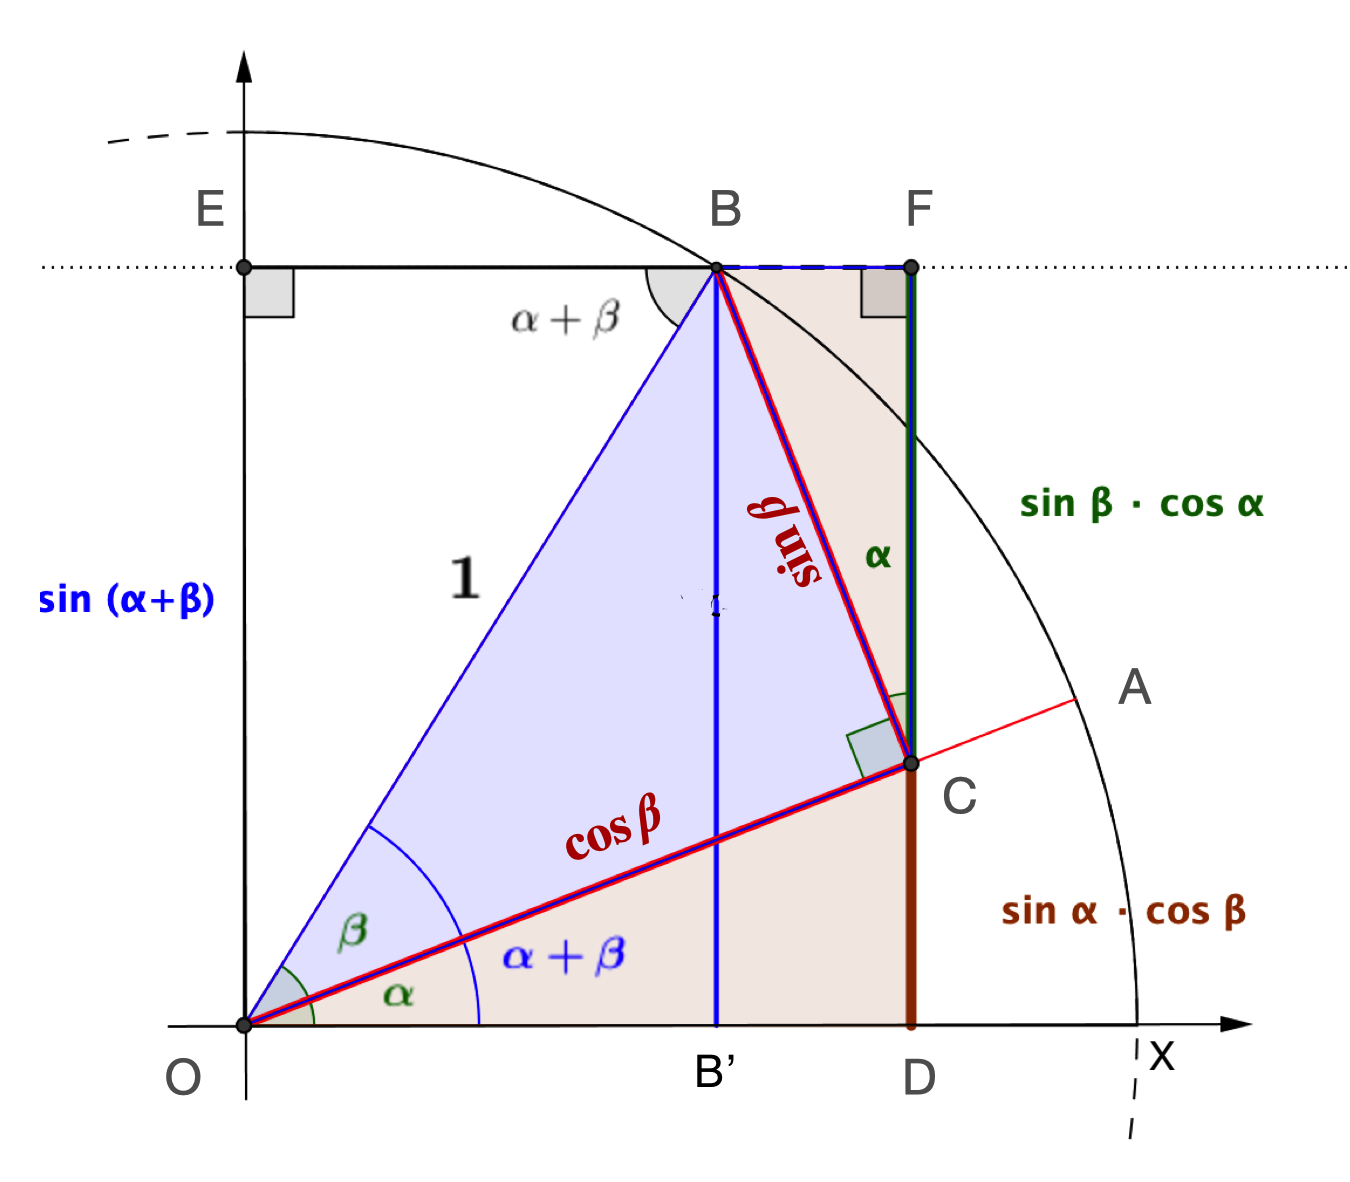
\includegraphics[width=.5\textwidth]{img-ft/ft02.png}
	\end{figure}

\vspace{-10mm}
En la circunferencia goniométrica dibujamos el ángulo $\alpha$ (arco XA) y, a partir de ahí, el ángulo $\beta$ (arco AB). Como consecuencia de dibujarlos consecutivos el arco XB repersenta al ángulo $\alpha + \beta$.

Proyectamos el punto B perpendicularmente sobre OA, obtenemos el punto de intersección C. Por construcción, el triángulo OCB es rectángulo en C, con hipotenusa OB=1, al estar B sobre la circunferencia goniométrica y ser O su centro. 

El ángulo opuesto al cateto BC es $\beta$, por lo que 
$\ \ \sin \beta=\dfrac{\text{cateto opuesto}}{\text{hipotenusa}}=\dfrac{CB}{1}=CB \ \ (*)\, . \ $ 

El cateto contiguo a $\beta$ en OCB es OC y, tendremos, $\ \ \cos \beta=\dfrac{\text{cateto contiguo}}{\text{hipotenusa}}=\dfrac {OC}{1}=OC \ \ (**)$

Trazamos la horizontal (paralela a OX) que pasa por B, corta al eje Y en el punto E. Trazamos la perpendicular (paralela al eje Y) que pasa por C, corta al eje X en el punto D y a la recta EB en el punto F.

Por construcción tenemos dos triángulos rectángulos, ODC (rectángulo en D) y BCF (rectángulo en F).

$\triangleright \ $ Triángulo ODC: la hipotenusa mide $OC=\cos \beta \ \ (**)\, . \ $ Estamos interesados en calcular el cateto opuesto al ángulo $\alpha\, , \ CD\, :$

$\sin \alpha=\dfrac{\text{cateto opuesto}}{\text{hipotenusa}} \ \to \ \text{cateto opuesto} =\text{hipotenusa} \cdot \sin \alpha= OC	\cdot \sin \alpha =\cos \beta \cdot \sin \alpha \ \to \ $

$\to \ \boldsymbol{CD=\cos \beta \cdot \sin \alpha}$  

$\triangleright \ $ Triángulo CBF: su hipotenusa mide $BC=\sin \beta \ \ (*)\, . \ $. El ángulo $C=\alpha$, ya que, por construcción, $FC \perp  OX$ y $BC \perp OA\,. \ $  Estamos interesados en calcular el cateto contiguo a $\alpha\, , \ CF\, :$

$\cos \alpha=\dfrac{\text{cateto contiguo}}{\text{hipotenusa}} \ \to \ \text{cateto contiguo} =\text{hipotenusa} \cdot \cos \alpha= CB \cdot \cos \alpha =\sin \beta \cdot \cos \alpha \ \to \ $

$\to \ \boldsymbol{CF=\sin \beta \cdot \cos \alpha}$  

Volviéndonos a fijar en la figura, en su ángulo total $\alpha + \beta$, su seno queda determinado por el segmento azul BB', $\ \sin(\alpha+\beta)=BB'\, , \ $ pero BB'=CD+CF por lo que, finalmente:

\vspace{5mm} \hspace{3cm} $ \boldsymbol{ \sin (\alpha + \beta) \ = \ \sin \alpha \, \cos \beta \ + \ \cos \alpha \, \sin \beta} $  \QED

Comprobemos que ahora sí funciona la fórmula en nuestro ejemplo inicial.


$\begin{cases} 
\ \sin (30+60)=\sin 90=1 \\
\ \sin 30  \cos 60 + \cos 30  \sin 60 =
\dfrac{1}{2} \dfrac{1}{2} + \dfrac{\sqrt 3}{4} \dfrac{\sqrt 3}{4}= \dfrac{1}{4}+\dfrac{3}{4}=1 \end{cases} \quad $ !Funciona!  \smiley{} 


\vspace{5mm} ------ Vamos ahora a por la fórmula correspondiente al coseno de la suma de ángulos.


\vspace{5mm}
\begin{theorem}[ Coseno de la suma de ángulos]

$$\boldsymbol{ \cos(\alpha+\beta) \ = \ \cos \alpha \, \cos \beta \ - \ \sin \alpha \, \sin \beta  }$$	
\end{theorem}

\underline{Demostración}:

\begin{figure}[H]
	\centering
	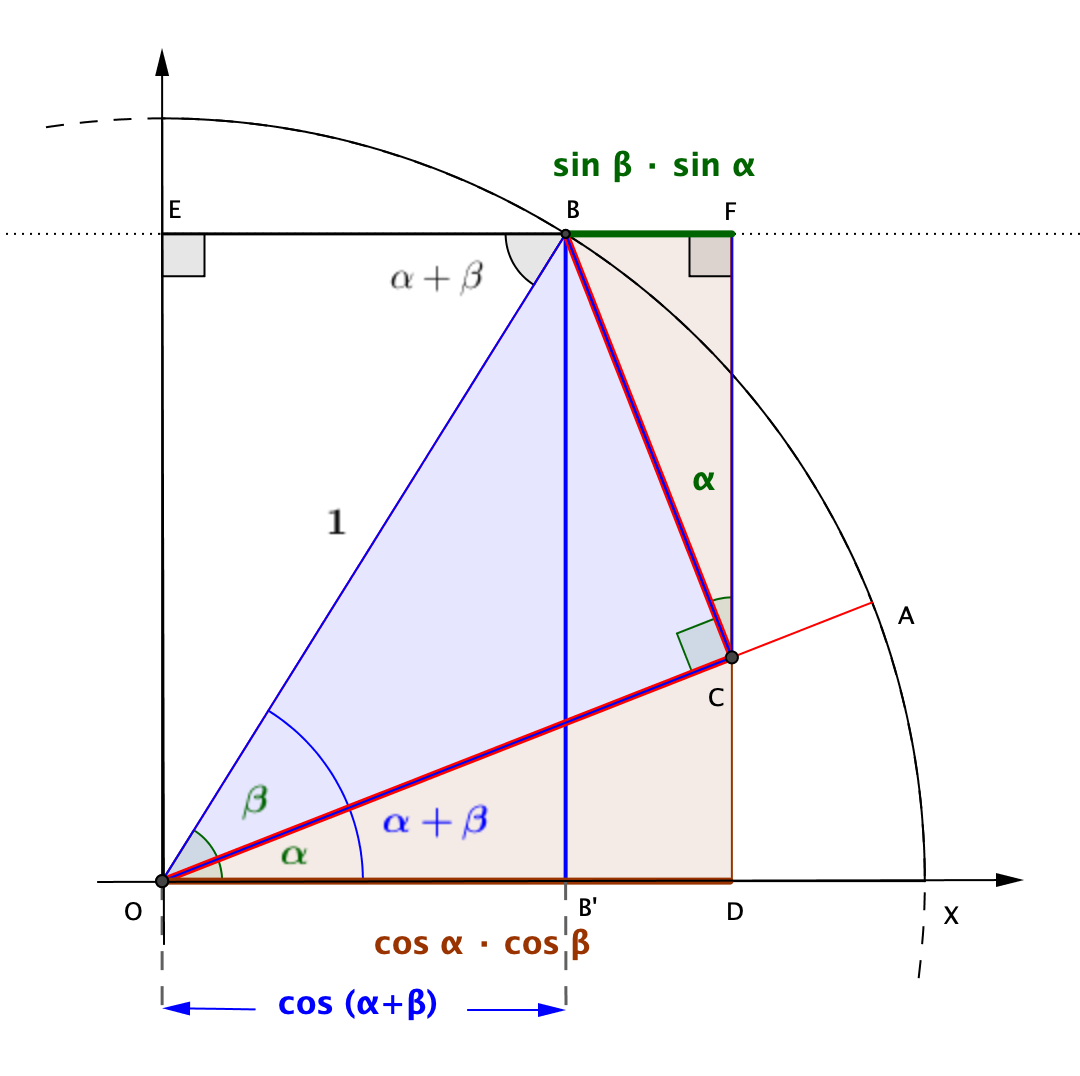
\includegraphics[width=.5\textwidth]{img-ft/ft03.png}
	\end{figure}

\vspace{-10mm}
Con la misma figura construida anteriormente, se observa que $\cos(\alpha+\beta)=OB'$, pero $OB'=OD-DB'$. Además, $DB'=FB$, por lo que $\cos(\alpha+\beta)=OD-FB$.

$\triangleright \quad$ Del triángulo $ODC \ \to \ \cos \alpha=\dfrac{OD}{\cos \beta} \ \to OD=\cos \alpha \cdot \cos \beta$

$\triangleright \quad$ Del triángulo $CFB \ \to \ \sin \beta=\dfrac{BF}{\sin \beta} \ \to \ FB=\sin \alpha \cdot \sin \beta$

Luego, $\ \ \boldsymbol{ \cos(\alpha+\beta) }=OD-FB=\boldsymbol{ \cos \alpha \, \cos \beta \ - \ \sin \alpha \, \sin \beta }$ \QED



\vspace{5mm} ------ Finalmente, la fórmula correspondiente a la tangente de la suma de ángulos.

\vspace{5mm}
\begin{theorem}[ Tangente de la suma de ángulos]

$$\boldsymbol{ \tan(\alpha+\beta) \ = \ \dfrac{\tan \alpha + \tan \beta}{1-\tan \alpha \cdot \tan \beta} }$$	
\end{theorem}

\underline{Demostración}:

$\tan(\alpha+\beta)=\dfrac{\sin (\alpha+\beta)}{\cos (\alpha+\beta)}= \dfrac{\sin \alpha \, \cos \beta + \ \cos \alpha \, \sin \beta}{\cos \alpha \, \cos \beta \ - \ \sin \alpha \, \sin \beta }= \ \to \ $ 
\textcolor{gris}{ (dividiendo numerador y denominador por } $\ \cos \alpha \cos \beta\, ) \  $
$\to \ = \dfrac{\dfrac{\sin \alpha \cancel{\cos \beta}}{\cos \alpha \cancel{\cos \beta}}+ \dfrac{\cancel{\cos \alpha} \sin \beta}{\cancel{\cos \alpha} \, \cos \beta} }{1-\dfrac{\sin \alpha \sin \beta}{\cos \alpha \cos \beta}}=\dfrac{\tan \alpha + \tan \beta}{1-\tan \alpha \cdot \tan \beta}$ \QED

\vspace{5mm}

\begin{miejemplo}

Calcula las RT del ángulo de $75^o$ \textcolor{gris}{$\qquad (75=30+45)$}

\vspace{4mm}
$\triangleright \quad \sin(75)=\sin(30+45)=\sin 30 \cos 45 + \cos 30 \sin 45= \dfrac 1 2 \dfrac{\sqrt{2}}{2}+\dfrac{\sqrt{3}}{2} \dfrac{\sqrt{2}}{2} = \dfrac{\sqrt{2}+\sqrt{6}}{4}$

\vspace{4mm}
$\triangleright \quad \cos(75)=\cos(30+45)=\cos 30 \cos 45 - \sin 30 \sin 45=\dfrac{\sqrt{3}}{2}\dfrac{\sqrt{2}}{2}-\dfrac 12 \dfrac{\sqrt{2}}{2}=\dfrac{\sqrt{6}-\sqrt{2}}{4}$

\vspace{4mm}
$\triangleright \quad \tan(75)=\tan(30+45)=\dfrac{\tan 30+\tan 45}{1-\tan 30\, \tan 45}=\dfrac{\dfrac{\sqrt{3}}{3}+1}{1-\dfrac{\sqrt{3}}{3}\, 1}=\dfrac{\sqrt{3}+1}{3-\sqrt{3}}=2+\sqrt{3}$

	
\end{miejemplo}




\vspace{5mm}
\begin{myalertblock}{Seno y cosenos de la suma de ángulos}
	%\begin{figure}[H]
	%\centering
	%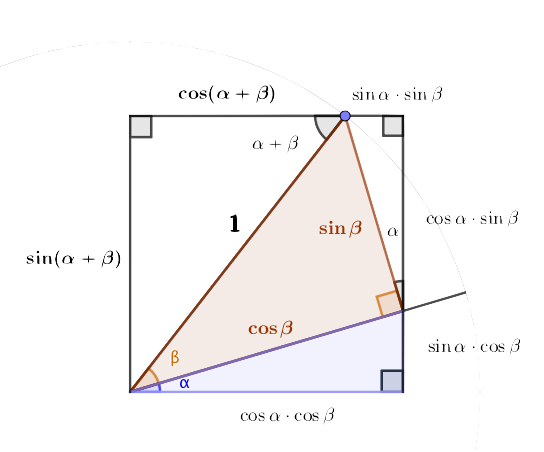
\includegraphics[width=.9\textwidth]{img-ft/ft01.png}
	%\end{figure}
	\begin{figure}[H]
	\centering
	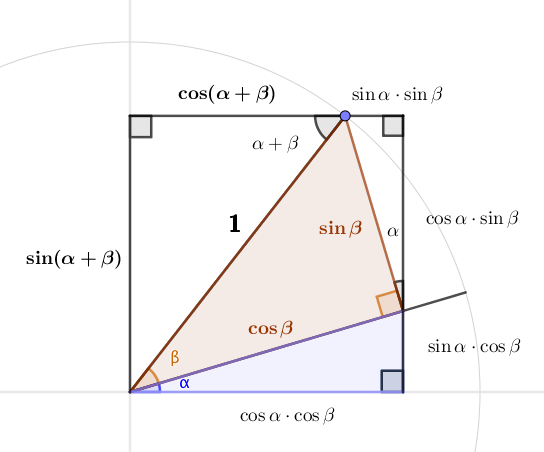
\includegraphics[width=.9\textwidth]{img-ft/ft01notransp.png}
	\end{figure}
	\vspace{2mm}
\end{myalertblock}



\newpage
\vspace{5mm}
\section{Razones trigonométricas de la resta de ángulos}

\begin{tikzpicture}
	\fill [left color=red!50, right color=teal!50] (0,0) rectangle (3.5,.1);
	\fill [left color=teal!50, right color=blue!50] (3.5,0) rectangle (7.5,.1);
	\end{tikzpicture}
\vspace{1cm}

Vamos a deducir las fórmulas para el seno, coseno y tangente de la resta de ángulos. Para ello nos basaremos en las propiedad de paridad de las funciones seno y coseno vistas en el tema anterior (también se puede interpretar como que los ángulos opuestos tienen los mismos cosenos y los senos opuestos) \textcolor{gris}{[ $x$ y $-x \, (=360-x)$ son opuestos ]}:

$$\subrayado{ \boldsymbol{ \sin (-x) \ = \ - \sin (x) \ ; \qquad \qquad  \cos (-x) \ = \ \cos (x)  \qquad \Rightarrow \quad \tan(-\alpha)=-\tan \alpha}} $$

Se obtienen las siguientes fórmulas:

\vspace{5mm}
\begin{theorem} [ RT de la diferencia de ángulos] 

$$ \boldsymbol{ \sin(\alpha-\beta) \ = \ \sin \alpha \, \cos \beta \ - \ \cos \alpha \, \sin \beta } $$

$$\boldsymbol{ \cos(\alpha - \beta) \ = \ \cos \alpha \, \cos \beta \ + \ \sin \alpha \, \sin \beta }$$

$$\boldsymbol{ \tan (\alpha - \beta) \ = \ \dfrac {\tan \alpha - \tan \beta}{1+\tan \alpha \, \tan \beta} }$$
 
\end{theorem}
\vspace{5mm} \underline{Demostraciones:}

Como hemos dicho, $\quad \sin(-\beta)=-\sin \beta\, ; \qquad \cos(-\beta)=\cos \beta$

\vspace{4mm} $\triangleright \quad \sin(\alpha-\beta)=\sin[\, \alpha +(-\beta)\, ]= \sin(\alpha)\cos(-\beta)+\cos(\alpha)\sin(-\beta) = \sin \alpha  \cos \beta  -  \cos \alpha  \sin \beta$ \QED

\vspace{4mm} $\triangleright \quad \cos(\alpha-\beta)=\cos[\,\alpha+(-\beta) \, ] = \cos(\alpha)\cos(-\beta) - \sin(\alpha)\sin(-\beta)=\cos \alpha  \cos \beta  +  \sin \alpha  \sin \beta$\QED

\vspace{4mm} $\triangleright \quad \tan(\alpha-\beta)=\tan [\, \alpha+(-\beta) \, ]= \dfrac{\tan(\alpha)+\tan(-\beta)}{1-\tan (\alpha) \, \tan(-\beta)}= \dfrac {\tan \alpha - \tan \beta}{1+\tan \alpha \, \tan \beta}$\QED

\vspace{5mm} \begin{miejemplo}
 . Calcula las RT de $\quad 15^0$ \textcolor{gris}{$\qquad (15=45-30)$}	

 \vspace{4mm} $\triangleright \quad \sin(15)=\sin(45-30)=\sin 45 \cos 30 - \cos 45 \sin 30= \dfrac{\sqrt{3}}{2} \dfrac{\sqrt{2}}{2}-\dfrac{\sqrt{2}}{2} \dfrac 1 2  = \dfrac{\sqrt{6}-\sqrt{2}}{4}$
 
 \vspace{4mm} $\triangleright \quad \cos(15)=\cos(45-30)=\cos 45 \cos 30 + \sin 45 \sin 30 = \dfrac{\sqrt{2}}{2} \dfrac{\sqrt{3}}{2} + \dfrac{\sqrt{2}}{2} \dfrac 1 2= \dfrac{\sqrt{6}+\sqrt{2}}{4}$
 
 \vspace{4mm} $\triangleright \quad \tan(15)=\tan(45-30)=\dfrac{\tan 45 - \tan 30}{1+\tan 45 \, \tan 30}= \dfrac{1- \dfrac{\sqrt{3}}{3} }{1+1\cdot \dfrac{\sqrt{3}}{3}}=\dfrac{3-\sqrt{3}}{3+\sqrt{3}}=2-\sqrt{3}$
 \end{miejemplo}

\vspace{5mm}Podemos escribir las fórmulas anteriores reducidas en:

\vspace{4mm}
\begin{adjustwidth}{10pt}{10pt}
\begin{destacado}
\vspace{-5mm} $$\boldsymbol{ \sin(\alpha\pm\beta)  =  \sin \alpha  \cos \beta  \pm \cos \alpha \sin \beta }\, ; \qquad \boldsymbol{ \cos(\alpha \pm \beta)  =  \cos \alpha  \cos \beta   \mp  \sin \alpha  \sin \beta }$$

\vspace{-5mm} $$\boldsymbol{ 
\tan (\alpha \pm \beta)  =  \dfrac {\tan \alpha \pm \tan \beta}{1 \mp \tan \alpha \, \tan \beta} }$$
\end{destacado}
\end{adjustwidth}

\vspace{3mm} \underline{Observación}: las fórmulas del seno y coseno de la suma y resta de ángulos  son aplicables a cualquier ángulo, pero no así la de tangentes. 
Para poder aplicar la fórmula de la tangente de suma o resta de ángulos es necesario que ambas tangentes estén definidas, que ni $\alpha$ ni $\beta$ sean múltiplos impares de $\pi/2$ \textcolor{gris}{$\left( \alpha \neq (2k+1)\dfrac \pi 2;\ \ \beta \neq (2k+1)\dfrac \pi 2;\ \ \forall k 	\in \mathbb Z \right)$}. Además, en la suma de ángulos $\tan \alpha \cdot \tan \beta \neq 1$ y en la resta $\tan \alpha \cdot \tan \beta \neq -1$, a fin de que no se anulen denominadores.

\vspace{5mm}
\section{Razones trigonométricas del ángulo doble}

\begin{tikzpicture}
	\fill [left color=red!50, right color=teal!50] (0,0) rectangle (3.5,.1);
	\fill [left color=teal!50, right color=blue!50] (3.5,0) rectangle (7.5,.1);
	\end{tikzpicture}
\vspace{1cm}

En esta ocasión nos interesa escribir $\ \sin 2\alpha,\ \ \cos 2\alpha,\ \ \tan 2\alpha \ $ en función de senos y cosenos del ángulo $\alpha$. Para ello, recurrimos a las formulas anteriores y haremos $\ \beta=	\alpha$.

\vspace{5mm} \begin{theorem} [ RT del ángulo doble]
 
 $$\boldsymbol{
\subrayado{\boxed{ \sin 2 \alpha \ = \ 2 \, \sin \alpha \, \cos \alpha} }\ ; \qquad \qquad 
\subrayado{\boxed{ \cos 2 \alpha \ = \ \cos^2 \alpha \ - \ \sin^2 \alpha}  }}$$

\vspace{-3mm} $$\subrayado{\boldsymbol{ \boxed{ \tan 2 \alpha \ = \ \dfrac{2\, \tan \alpha}{1\, - \, \tan^2 \alpha}}}}$$
 \end{theorem}

\underline{Demostraciones}

\vspace{4mm} $\triangleright \quad \sin 2\alpha =\sin (\alpha + \alpha)= \sin \alpha \cos \alpha + \cos \alpha \sin \alpha = 2\sin \alpha \cos \alpha$ \QED

\vspace{4mm} $\triangleright \quad \cos 2\alpha=\cos (\alpha + \alpha)= \cos \alpha \cos \alpha - \sin \alpha \sin \alpha = \cos^2 \alpha - \sin2 \alpha$ \QED

\vspace{4mm} $\triangleright \quad \tan 2 \alpha= \tan (\alpha + \alpha)= \dfrac{\tan \alpha + \tan \alpha}{1-\tan \alpha \cdot \tan \alpha}=\dfrac{2\tan \alpha}{1-\tan^2 \alpha}$ \QED

\vspace{3mm} \underline{Observaciones}: La fórmula para la tangente del ángulo doble no se puede aplicar en el caso en que $\tan \alpha=\pm 1$, ya que anula el denominador. \textcolor{gris}{Esto ocurre cuando el ángulo es múltiplo impar de 45$^o$, ha de ocurrir pues que $\alpha \neq (2k+1)\dfrac \pi 4,\ \ \forall k\in \mathbb Z \, . \ $ Además, obviamente $\tan \alpha$ ha de estar definida, por lo que $\alpha \neq (2k+1)\frac \pi 2$.}

\vspace{5mm}

\begin{miejemplo}

Calcula las RT de $60^o$ a partir de las de $30^o$


\vspace{4mm} $\triangleright \quad  \sin 60=\sin(2\cdot 30)=2\, \sin 30\, \cos 30=2\, \dfrac 1 2 \dfrac {\sqrt{3}}{2}=\dfrac {\sqrt{3}}{2} $

\vspace{4mm} $\triangleright \quad  \cos 60=\cos(2\cdot 30)=\cos^2 30-\sin^2 30= \left( \dfrac {\sqrt{3}}{2} \right)^2-\left( \dfrac {\sqrt{1}}{2} \right)^2=\dfrac 3 4 - \dfrac 1 4 = \dfrac 1 2$

\vspace{4mm} $\triangleright \quad  \tan 60=\tan(2\cdot 30)=\dfrac{2\tan 30}{1-\tan^2 30}=\dfrac{2\,  \dfrac {\sqrt{3}}{3} }{1- \left( \dfrac {\sqrt{3}}{3} \right)^2}=\dfrac{ \dfrac {2\sqrt{3}}{3}}{\dfrac 2 3}=\sqrt{3}$


\end{miejemplo}



\vspace{5mm}
\section{Razones trigonométricas del ángulo mitad}

\begin{tikzpicture}
	\fill [left color=red!50, right color=teal!50] (0,0) rectangle (3.5,.1);
	\fill [left color=teal!50, right color=blue!50] (3.5,0) rectangle (7.5,.1);
	\end{tikzpicture}
\vspace{1cm}


Ahora nos interesa escribir $\ \sin (\alpha/2),\ \ \cos (\alpha/2),\ \ \tan (\alpha/2) \ $ en función de senos y cosenos del ángulo $\alpha$. Para ello, combinaremos adecuadamente la relación fundamental de la trigonometría, $\boldsymbol{\sin^2 \alpha+\cos^2 \alpha=1}$ con el coseno del ángulo doble, $\boldsymbol{\cos^2 \alpha - \sin^2 \alpha = \cos 2\alpha}$

\vspace{5mm}
\begin{theorem} [ RT del ángulo mitad]

$$\boldsymbol{ 
\subrayado{\boxed{ \sin \dfrac \alpha 2 \ = \ \pm\sqrt{\dfrac{1-\cos \alpha}{2}} }}  \qquad 
\subrayado{\boxed{ \cos \dfrac \alpha 2 \ = \ \pm\sqrt{\dfrac{1+\cos \alpha}{2}} }}  \qquad 
\subrayado{\boxed{ \tan \dfrac \alpha 2 \ = \ \pm\sqrt{\dfrac{1-\cos \alpha}{1+\cos \alpha}} }}  
}$$
\end{theorem}

\underline{Demostraciones}:

$\begin{cases}
\ \cos^2 \alpha + \sin^2 \alpha = 1 \\
\ \cos^2 \alpha - \sin^2 \alpha = \cos 2\alpha 	
\end{cases} \ \Rightarrow \ \begin{array}{lll}
\text{ sumando} & 2\cos^2\alpha=1+\cos 2 \alpha  & \to \ \cos \alpha=\sqrt{\dfrac{1+\cos 2\alpha}{2}}	 \\
\text{ restando} & 2\sin^2\alpha=1-\cos 2 \alpha  & \to \ \sin \alpha=\sqrt{\dfrac{1-\cos 2\alpha}{2}}	
 \end{array}$
 
 Solo nos queda intercambiar los ángulos $\ \alpha \ \leftrightarrow \ \dfrac \alpha 2$, para obtener los resultados buscados:

$\cos \dfrac \alpha 2 =\pm \sqrt{\dfrac{1+\cos \alpha}{2}}\, ; \qquad 
\sin \dfrac \alpha 2 =\pm \sqrt{\dfrac{1-\cos \alpha}{2}}$

Finalmente, para la $\tan \alpha/2$ solo tenemos que dividir ambas expreiones:

$\tan \dfrac \alpha 2=\dfrac{\sin \dfrac \alpha 2}{\cos \dfrac \alpha 2}=\pm \sqrt{\dfrac{1-\cos \alpha}{1+\cos \alpha}}$ \QED
 
\vspace{3mm} \underline{Observaciones}: El doble signo en las fórmulas de las RT del ángulo mitad quedará determinado al conocer el cuadrante al que pertenezca el ángulo $\dfrac \alpha 2$.
 
\vspace{5mm}

\begin{miejemplo}

Calcula las RT de $30^o$ a partir de las de $60^o$


\vspace{4mm} $\triangleright \quad  \sin 30 =\sin \dfrac{60}{2}= \pm\sqrt{\dfrac{1-\cos 60}{2}}=\pm\sqrt{\dfrac{1-\dfrac 12}{2}}=\pm\sqrt{\dfrac 1 4}=\dfrac 12$
			
\vspace{4mm} $\triangleright \quad  \cos 30=\cos \dfrac {60} 2=\pm \sqrt{ \dfrac{1+\cos 60}{2} }= \pm\sqrt{\dfrac{1+\dfrac 12}{2}}=\pm \sqrt{\dfrac{3}{4}}=\dfrac{\sqrt{3}}{2}$

\vspace{4mm} $\triangleright \quad  \tan 30= \tan \dfrac {60} 2=\pm \sqrt
{\dfrac{1-\cos 60}{1+\cos 60}}=\pm \sqrt
{\dfrac{1-\dfrac 1 2}{1+\dfrac 12}}=\pm\sqrt{\dfrac{1/2}{1/3}}=\dfrac{1}{\sqrt{3}}=\dfrac{\sqrt{3}}{3}$


\end{miejemplo}



\vspace{4mm}
\section{Transformación de sumas en productos}

\begin{tikzpicture}
	\fill [left color=red!50, right color=teal!50] (0,0) rectangle (3.5,.1);
	\fill [left color=teal!50, right color=blue!50] (3.5,0) rectangle (7.5,.1);
	\end{tikzpicture}
\vspace{7mm}

En esta ocasión buscamos poder transformar la suma o resta de dos senos (o de dos cosenos) en un producto de RT, con objeto de poder simplificar cuando aparezcan expresiones de este tipo en cocientes. 

\vspace{4mm}
\begin{theorem} [ Transformación de sumas (restas) en productos]

\begin{multicols}{2}

$\subrayado{\boxed{ \ \boldsymbol{  \sin \alpha + \sin \beta \ = \ 2 \, \sin \dfrac{\alpha + \beta}{2}\, \cos \dfrac{\alpha - \beta}{2} }  \ }}$

\vspace{3mm} $\subrayado{\boxed{ \ \boldsymbol{ \cos \alpha + \cos \beta \ = \ 2 \, \cos \dfrac{\alpha + \beta}{2}\, \cos \dfrac{\alpha - \beta}{2} }  \ }}$

$\subrayado{\boxed{ \ \boldsymbol{ \sin \alpha - \sin \beta \ = \ 2 \, \cos \dfrac{\alpha + \beta}{2}\, \sin \dfrac{\alpha - \beta}{2}  }  \ }}$

\vspace{3mm} $\subrayado{\boxed{ \ \boldsymbol{  \cos \alpha - \cos \beta \ = \ - 2 \, \sin \dfrac{\alpha + \beta}{2}\, \sin \dfrac{\alpha - \beta}{2} }  \ }}$
	
\end{multicols}
	
\end{theorem}

\underline{Demostraciones}:

 Las demostraciones se obtienen al combinar las fórmulas del seno de la suma y de la resta de ángulos y las fórmulas del coseno de la suma y resta de ángulos.
 
 $\begin{cases}
\ \sin(\alpha+\beta)=\sin \alpha \cos \beta + \cos \alpha \sin \beta \\	
\ \sin(\alpha-\beta)=\sin \alpha \cos \beta - \cos \alpha \sin \beta 
\end{cases} \ \to \ $

\hspace{5cm} $\to \ \  \begin{array}{ll}
 	\text{sumando:}&\sin(\alpha+\beta)+\sin(\alpha-\beta)=2\sin\alpha \cos \beta     \ \ (1*)\\ \text{restando:}&\sin(\alpha+\beta)-\sin(\alpha-\beta)=2\cos\alpha \sin \beta  \ \ (2*)
 \end{array}$
                                         

 
\vspace{3mm} $\begin{cases}
\ \cos(\alpha+\beta)=\cos \alpha \cos \beta - \sin \alpha \sin \beta \\	
\ \cos(\alpha-\beta)=\cos \alpha \cos \beta + \sin \alpha \sin \beta  
\end{cases} \ \to \ $

\hspace{5cm} $\to \ \  \begin{array}{ll}
 	\text{sumando:}&\cos(\alpha+\beta)+\cos(\alpha-\beta)=2\cos\alpha \cos \beta \ \ (3*) \\ \text{restando:}&\cos(\alpha+\beta)-\cos (\alpha-\beta)=-2\sin\alpha \sin \beta \ (4*)
 \end{array}$
 
\vspace{3mm} Llamando $\ \begin{cases} \ \alpha + \beta =A\\ \ \alpha - \beta=B \end{cases} \ \to \ \begin{cases} \ 2\alpha=A+B \\ \ 2\beta=A-B \end{cases} \ \to \ \begin{cases} \ \alpha= \dfrac{A+B}{2} \\   \ \beta= \dfrac{A-B}{2} \end{cases}$


Incorporando estos resultados a las ecuaciones $(1*),\, (2*),\, (3*) \text{ y }  
 (4*)\, , \ $ se obtienen los resultados que andamos buscando. \QED

\vspace{5mm} 
\begin{miejemplo}

Sin usar calculadora, encuentra el valor de $\ \sin 75^o-\sin 15^o$	

\vspace{5mm}
$\sin 75-\sin 15= 2 \, \cos \left( \dfrac{75+15}{2} \right) \, \sin \left( \dfrac{75-15}{2} \right) = 2\, \cos 45 \ \sin 30 = 2\dfrac{\sqrt{2}}{2}\dfrac 12=\dfrac {\sqrt{2}}{2}$
\end{miejemplo}


\vspace{10mm} \begin{large}
 \textbf{Transformación de productos en sumas}	
 \end{large}
 
 Las mismas expresiones antes mencionadas,  $(1*),\, (2*),\, (3*) \text{ y }  
 (4*)\, , \ $, que hemos obtenido al demostrar las fórmulas de transformación de sumas en productos, nos sirven para expresar productos como sumas. Esto será muy útil a la hora de integrar (algo que se verá en cálculo avanzado).



\vspace{5mm}

\begin{adjustwidth}{100pt}{75pt}
\begin{destacado}
$(1*) \ \to \ \sin\alpha \cos \beta = \dfrac 1 2 \left( \sin(\alpha+\beta)+\sin(\alpha-\beta) \right)$

$(2*) \ \to \ \cos\alpha \sin \beta  =\dfrac 1 2 \left(  \sin(\alpha+\beta)-\sin(\alpha-\beta) \right)$

$(3*) \ \to \ \cos\alpha \cos \beta =\dfrac 1 2 \left(  \cos(\alpha+\beta)+\cos(\alpha-\beta) \right)$

$(4*) \ \to \ \sin\alpha \sin \beta =-\dfrac 1 2 \left(   \cos(\alpha+\beta)-\cos (\alpha-\beta) \right)$
\end{destacado}
\end{adjustwidth}


\vspace{5mm}
\begin{myexampleblock}{Nemotécnia para recordar las fórmulas}
\vspace{-5mm}
 $$\boldsymbol{ \sin(\alpha\pm\beta)  =  \sin \alpha  \cos \beta  \pm \cos \alpha \sin \beta }\, ; \qquad \boldsymbol{ \cos(\alpha \pm \beta)  =  \cos \alpha  \cos \beta   \mp  \sin \alpha  \sin \beta }$$
 
 \begin{itemize}
 \item \underline{seno de la suma} (resta) es igual a \textbf{seno coseno más} (menos) \textbf{coseno seno}.
 \item \underline{coseno de la suna} (resta) es igual a \textbf{coseno coseno menos} (más) \textbf{seno seno	}.
 \end{itemize}


\vspace{-3mm} $$\boldsymbol{ 
\tan (\alpha \pm \beta)  =  \dfrac {\tan \alpha \pm \tan \beta}{1 \mp \tan \alpha \, \tan \beta} }$$

\begin{itemize}
\item \underline{tangente de la suma} (resta) es igual a \textbf{tangente más} (menos) \textbf{tangente dividido entre uno menos} (más) \textbf{tangente por tangente}.	
\end{itemize}

 $$\boldsymbol{
 \sin 2 \alpha \ = \ 2 \, \sin \alpha \, \cos \alpha\ ; \qquad \qquad 
 \cos 2 \alpha \ = \ \cos^2 \alpha \ - \ \sin^2 \alpha}  $$
 
 \begin{itemize}
 \item \underline{seno del ángulo doble} es \textbf{dos seno coseno}.
 \item \underline{coseno del ángulo doble} es \textbf{coseno al cuadrado menos seno al cuadrado}.	
 \end{itemize}


\vspace{-3mm} $$\boldsymbol{  \tan 2 \alpha \ = \ \dfrac{2\, \tan \alpha}{1\, - \, \tan^2 \alpha}}$$

\begin{itemize}
\item \underline{tangente del ángulo doble} es \textbf{dos tangente entre uno menos la tangente al cuadrado	}.
\end{itemize}

\vspace{-3mm}
$$\boldsymbol{ 
 \sin \dfrac \alpha 2 \ = \ \pm\sqrt{\dfrac{1-\cos \alpha}{2}}  \qquad 
 \cos \dfrac \alpha 2 \ = \ \pm\sqrt{\dfrac{1+\cos \alpha}{2}}  \qquad 
 \tan \dfrac \alpha 2 \ = \ \pm\sqrt{\dfrac{1-\cos \alpha}{1+\cos \alpha}}   
}$$

\begin{itemize}
\item \underline{seno ángulo mitad} es \textbf{más menos la raiz de 1 menos coseno, entre dos}.	
\item \underline{coseno ángulo mitad} es \textbf{más menos la raiz de 1 más coseno, entre dos}.
\item \underline{tangente ángulo mitad} es \textbf{más menos la raiz de 1 menos coseno, entre 1 más coseno}.
\end{itemize}


\vspace{3mm}
\begin{multicols}{2}

$\ \boldsymbol{  \sin \alpha + \sin \beta \ = \ 2 \, \sin \dfrac{\alpha + \beta}{2}\, \cos \dfrac{\alpha - \beta}{2} }  \ $

\vspace{3mm} $ \ \boldsymbol{ \cos \alpha + \cos \beta \ = \ 2 \, \cos \dfrac{\alpha + \beta}{2}\, \cos \dfrac{\alpha - \beta}{2} }  \ $

$ \ \boldsymbol{ \sin \alpha - \sin \beta \ = \ 2 \, \cos \dfrac{\alpha + \beta}{2}\, \sin \dfrac{\alpha - \beta}{2}  }  \ $

\vspace{3mm} $ \ \boldsymbol{  \cos \alpha - \cos \beta \ = \ - 2 \, \sin \dfrac{\alpha + \beta}{2}\, \sin \dfrac{\alpha - \beta}{2} }  \ $
\end{multicols}

\begin{itemize} 
\item \underline{suma de senos} es \textbf{dos veces el seno de la semisuma por el coseno de la semidiferencia}.
\item \underline{resta de senos} es \textbf{dos veces el coseno de la semisuma por el seno de la semidiferencia}.
\item \underline{suma de cosenos} es \textbf{dos veces el coseno de la semisuma por el coseno de la semidiferencia}.	
\item \underline{resta de cosenos} es menos \textbf{dos veces el seno de la semisuma por el seno de la semidiferencia}.	
\end{itemize}

\end{myexampleblock}




\vspace{5mm}
\section{Identidades y ecuaciones trigonométricas (II/II)}

\begin{tikzpicture}
	\fill [left color=red!50, right color=teal!50] (0,0) rectangle (3.5,.1);
	\fill [left color=teal!50, right color=blue!50] (3.5,0) rectangle (7.5,.1);
	\end{tikzpicture}
\vspace{1cm}

Las ecuaciones trigonométicas se reducirán a uno de estos tres tipos:

\vspace{3mm}
\begin{table}[H]
\centering
\begin{tabular}{l|c|c|c|}
\cline{2-4}
 &  Tipo seno & Tipo coseno & Tipo tangente  \\ \hline
\multicolumn{1}{|l|}{Ecuación:} & $\sin x=a$ & $\cos x=a$ & $\tan x=a$ \\ \hline
\multicolumn{1}{|l|}{Con calculadora:} & $x=\asin a$ & $x=\acos a$  &  $x=\atan a$ \\ \hline
\multicolumn{1}{|l|}{$\mqty{\text{Solución general, \quad \ \ } \\ \text{si estamos con grados}}$} & $\mqty{ x_1=x+360k \\ x_2=(180-x)+360k }$ & $\mqty{ x_1=x+360k \\ x_2=(360-x)+360k }$ & $\mqty{ x_1=x+360k \\ x_2=(180+x)+360k }$ \\ \hline
\multicolumn{1}{|l|}{$\mqty{\text{Solución general, \quad \quad \ \ } \\ \text{si estamos con radianes}}$} & $\mqty{ x_1=x+2k\pi \\ x_2=(\pi-x)+2k\pi}$ & $\mqty{ x_1=x+2k\pi \\ x_2=(2\pi-x)+2k\pi}$ & $\mqty{ x_1=x+2k\pi \\ x_2=(\pi+x)+2k\pi}$ \\ \hline
\end{tabular}
\end{table}


De todos modos y tal y como dijimos en el capítulo anterior, no es preciso memorizar todo esto, solo entenderlo y, en cada caso, dibujar los ángulos que pueden ser solución.

\vspace{5mm}

\begin{miejemplo}

Simplifica las expresiones $\ \ a)\ \ \dfrac{\tan(a+b)-\tan a}{1+\tan(a+b)\tan a} \, ; \qquad \qquad b) \cos(270-a)-\cos(90-a)$	

\vspace{5mm} $\triangleright \quad a) \ $ Procedimiento largo, sustituyamos $\tan(a+b)$ por su fórmula adecuada.

\vspace{2mm} $ \dfrac{\tan(a+b)-\tan a}{1+\tan(a+b)\tan a} =  
\dfrac{\dfrac{\tan a+\tan b}{1-\tan a \tan b} -\tan a}{1+ \dfrac{\tan a+\tan b}{1-\tan a \tan b} \, \tan a} = \ \cdots \ = \tan a$

\vspace{2mm} Un procedimiento más abreviado consistiría en identificar que en el ejercicio en cuestión está la fórmula de la tangente de la resta de ángulos \textcolor{gris}{(tangente menos tangente dividido por uno más tangente por tangente)}, siendo $a + b$ y $a$ los ángulos que intervienen.

\vspace{2mm} $\dfrac{\tan(a+b)-\tan a}{1+\tan(a+b)\tan a} = \tan [ (a+b) - (a) ] = \tan a$


\vspace{5mm} $\triangleright \quad b)\ $ Hay múltiples formas de resolver este ejercicio (incluso podría resolverse en el tema pasado), per vamos a transformar esta resta en productos \textcolor{gris}{(coseno menos coseno es igual a menos dos veces el seno de la semisuma por el seno de la semidiferencia).}

\vspace{2mm}  $\cos(270-a)-\cos(90-a) = -2 \, \sin \left( \dfrac {(270-a)+(90-a)}{2} \right) \, \sin \left( \dfrac {(270-a)-(90-a)}{2} \right) = -2 \sin (180-a) \cancelto{1}{\sin 90}= -2\sin(180-a) = \ \to $

\vspace{2mm} Ahora, podríamos hacer uso de ángulos suplementarios o, como estamos en el tema de fórmulas, usaremos el seno de la resta de ángulos.

\vspace{2mm} $\to \ = -2 \left( \cancelto{0}{\sin 180} \cos a - \cancelto{-1}{\cos 180} \sin a \right)=-2(0-(-1)\sin a)=-2\sin a$
\end{miejemplo}

\vspace{5mm}
\begin{cuadro-naranja}
\textbf{Pautas} generales para resolver ecuaciones trigonométricas:
\begin{adjustwidth}{20pt}{20pt}
\begin{itemize}
\item Los argumentos de las RT que intervengan deben de ser todos iguales.	
\item Se pueden transformar sumas y restas de senos o cosenos en productos si interesa, por ejemplo si están igualadas a cero (tendríamos un producto igual a cero).
\item Al final, la ecuación debe contener una única razón trigonométrica (senos, cosenos o tangentes).
\end{itemize}
\end{adjustwidth}
\end{cuadro-naranja}

\vspace{5mm}

\begin{miejemplo}

Resuelve las ecuaciones. $\quad a)\ \ \sin x-\sin 2x=0;\qquad b)\ \sin 4x - \sin 2x=0$	

\vspace{5mm} $\triangleright \quad a)\ \ \sin x - \sin 2x=0\quad $ Usamos la fórmula del seno del ángulo doble \textcolor{gris}{(seno del ángulo doble es dos veces el seno por el coseno)} .

\vspace{2mm} $\sin x-2\sin x\ cos x=\sin x(1-2\cos x)=0 \to \begin{cases}
 	\ \sin x=0 & \to \ \begin{cases} \ x=0+360k \\ \ x=180+360k \end{cases} \\
 	\ \cos x=\dfrac 1 2 &\to \begin{cases} \ x=60+360k \\ x=300+360 k \end{cases}
 	 \end{cases}$


\vspace{5mm} $\triangleright \quad b)\ \ \sin 4x - \sin 2x=0\quad$ Transformamos en productos \textcolor{gris}{(seno menos seno es dos veces coseno de la semisuma seno semidiferencia)}. 

\vspace{2mm} $\sin 4x - \sin 2x=2\, \cos 3x \, sin x =0 \ \to \begin{cases}
\ \sin x=0 & \to \ \begin{cases} \ x=0+360k \\ \ x=180+360k \end{cases} \\
\ \cos 3x=0 & \to  \ \begin{cases}  \ 3x=90+360 k  & \to x=30+120 k\\ \ 3x=270+360k & \to x=90+120k \end{cases}	
 \end{cases}$

\vspace{2mm} \underline{Nótese} que las últimas soluciones tienen un término $120k$. Para buscar todas las soluciones en la primera vuelta, en $[0,360[$, las posibilidades son: $x=30+120k \to 20,\, 150,\, 270\;\ $ y $x=90+120k \to 90,\, 210,\, 330$, que junto con las otras dos soluciones anteriores, $x=0$ y $x=180$ y una vez ordenadas y generalizadas para cualquier número de vueltas queda que la solución general de esta ecuación es:

\vspace{2mm} $x=0+360k, \ \ x=30+360k, \ \ x=90+360k,\ \ x=150+360k,\ \ x=180+360k,\ \ x=210+360k,\ \ x=270+360k,\  \text{ y } \ x=330+360 k$

\end{miejemplo}



\vspace{5mm}
\begin{myalertblock}{Cambio trigonométrico general en integración}

Vamos a escribir el $\ \sin x,\ \cos x,\ \tan x\ $	en función de $\ \tan \dfrac x 2\ $. Este cambio de variable no es caprichoso, se usará en la integración de funciones racionales trigonométricas como cambio general (en cálculo avanzado).

\vspace{2mm}Empezamos llamando $\ \boldsymbol{\tan \dfrac x 2 \ = \ t } \ $ y construyendo nuestro triángulo rectángulo \emph{ad hoc}.

\begin{figure}[H]
	\centering
	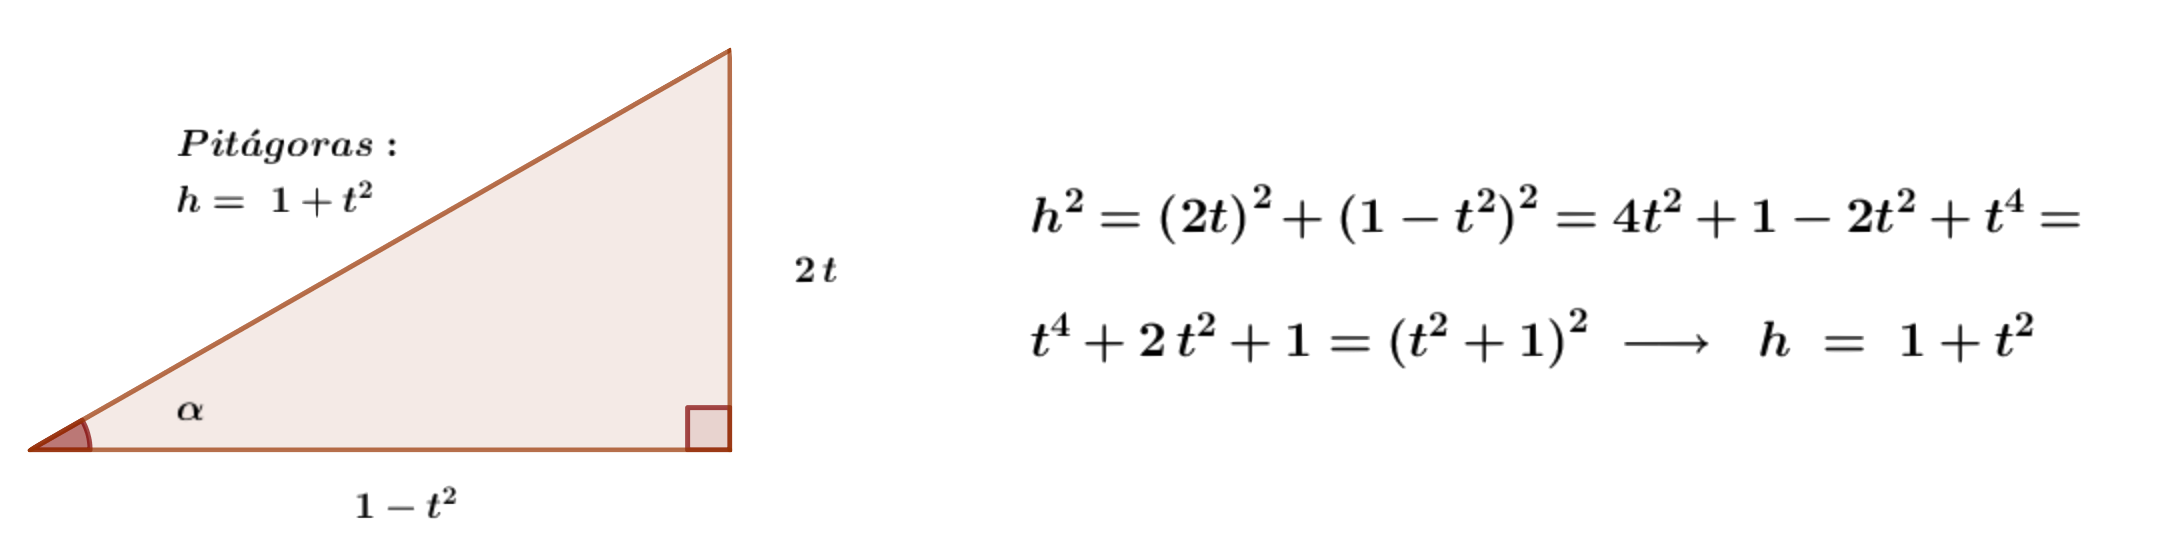
\includegraphics[width=.95\textwidth]{img-ft/ft08.png}
	\end{figure}
	
\hspace{2cm} \vspace{2mm} $\boldsymbol{ \tan x} = \tan \left( 2 \, \dfrac x 2 \right) = \dfrac{2 \tan \dfrac x 2}{1-\tan^2 \dfrac x 2} = \dfrac{2t}{1-t^2}\quad $ De la figura, 

\hspace{2cm} \vspace{2mm} $\boldsymbol{ \sin x} = \dfrac{2t}{1+t^2}=\dfrac{2 \tan \dfrac x 2}{1+\tan^2 \dfrac x 2} \qquad \qquad \boldsymbol{\cos x}=\dfrac{1-t^2}{1+t^2}=\dfrac{1-\tan^2 \dfrac x 2}{1+\tan^2 \dfrac x 2}$ 
\end{myalertblock}

%\vspace{5mm}
\begin{figure}[H]
	\centering
	
\includegraphics[width=.6\textwidth]{img-ft/ft04.png}
	\end{figure}
	
\vspace{1cm}%%%%%
\section{Ejercicios}

\begin{tikzpicture}
	\fill [left color=red!50, right color=teal!50] (0,0) rectangle (3.5,.1);
	\fill [left color=teal!50, right color=blue!50] (3.5,0) rectangle (7.5,.1);
	\end{tikzpicture}
\vspace{0.5cm}

%*****************
\begin{miejercicio}

Sabiendo que $\ \cot \alpha=-2\ $ y que $\ \sin \beta=4\cos \beta\, , \ $ calcula $\ \tan (\alpha-\beta) $ y $\ \tan 2\alpha$ 

\rule{250pt}{0.1pt}

\vspace{4mm}

$\triangleright \quad \cot \alpha=-2\ \to \tan \alpha = -1/2\, ; \quad a $ 
$\sin \beta=4\cos \beta \ \to \tan \beta= 4 \quad \Rightarrow $	

\vspace{2mm} \hspace{2cm} $\Rightarrow \quad \tan (\alpha-\beta)= \dfrac{\tan \alpha - \tan \beta}{1+\tan \alpha \, \tan \beta} = \dfrac{(-1/2)-(4)}{1+(-1/2)(4)}=9/2$

\vspace{2mm}  $\triangleright \quad \tan 2 \alpha = \dfrac{2\tan \alpha}{1-\tan^2 \alpha}=\dfrac{2(-1/2)}{1-(-1/2)^2}=-4/3$


\end{miejercicio}


%*****************
\begin{miejercicio}

$\alpha \in \text{II-cuadrante, con } \ \sin \alpha=1/3\, , \ $ calcula:

\vspace{2mm} \hspace{2cm} $a)\ \ \sin 2 \alpha;\quad b)\ \  \sin \dfrac \alpha 2 ;\quad c)\ \ \cos (\pi+\alpha) ;\quad d)\ \ \tan(\pi-\alpha)$

\rule{250pt}{0.1pt}

\vspace{4mm} Relación fundamental: $\quad \sin^2 \alpha + \cos^2 \alpha = 1 \ \to \ \cos \alpha=-2\dfrac{\sqrt{2}}{2}; \quad \tan \alpha=-\dfrac{\sqrt{2}}{4}$

\vspace{4mm} $\triangleright \ \ a)\ \ \sin 2 \alpha= 2\sin \alpha \cos \alpha= \cdots \cdots = -\dfrac{4\sqrt{2}}{9}$
	


\vspace{4mm} $\triangleright \ \ b)\ \ \sin \dfrac \alpha 2 = \pm \sqrt{\dfrac{1-\cos \alpha}{2}}= \cdots \cdots = \sqrt{\dfrac{3+2\sqrt{2}}{6}}$



\vspace{4mm} $\triangleright \ \ c)\ \ \cos (\pi+\alpha)= \cos \pi \cos \alpha -\sin \pi \sin \alpha= \cdots \cdots = 2\dfrac{\sqrt{2}}{3}$



\vspace{4mm} $\triangleright \ \ d)\ \ \tan (\pi-\alpha)= \dfrac{\tan \pi + \tan \alpha}{1+\tan \pi \, \tan \alpha}=\cdots \cdots =\dfrac{\sqrt{2}}{4}$




\end{miejercicio}


%*****************
\begin{miejercicio}

Calcula: $\qquad \dfrac{\sin 40 + \sin 20}{\cos 40 + \cos 20}$

\rule{250pt}{0.1pt}

\vspace{4mm}
	
Transformando en productos, $\ \ \dfrac{\sin 40 + \sin 20}{\cos 40 + \cos 20}= \dfrac{2\sin 30 \cos 10}{2\cos 30 \cos 10}=\tan 30= \dfrac{\sqrt{3}}{3}$
\end{miejercicio}


%*****************
\begin{miejercicio}

Demuéstrese que $\quad \cos(\alpha+\beta)\ \cos(\alpha-\beta)= \cos^2 \beta-\sin^2 \alpha$

\rule{250pt}{0.1pt}

\vspace{4mm}	
$\cos(\alpha+\beta)\ \cos(\alpha-\beta) = (\cos \alpha \cos \beta - \sin \alpha \sin \beta)\, (\cos \alpha \cos \beta + \sin \alpha \sin \beta)=$


\vspace{2mm} $=(\cos \alpha \cos \beta)^2 - (\sin \alpha \sin \beta)^2=  \cos^2 \alpha \cos^2 \beta - \sin^2 \alpha \sin^2 \beta= $

\vspace{2mm} $=(1-\sin^2 \alpha) \cos^2 \beta - \sin^2 \alpha (1-\cos^2 \beta)=
\cos^2 \beta- \cancel{\sin^2 \alpha \ cos^2 \beta} -\sin^2 \alpha +\cancel{\sin^2 \alpha \cos^2 \beta} = $

\vspace{2mm} $= \cos^2 \beta - \sin^2 \alpha$ \textcolor{gris}{\QED}
\end{miejercicio}


%*****************
\begin{miejercicio}

Demuéstrese que $\qquad \dfrac{1-\tan a}{1+\tan a}=\dfrac{1-\sin2 a}{\cos2 a}$

\rule{250pt}{0.1pt}

\vspace{4mm}
	$\dfrac{1-\tan a}{1+\tan a}=\dfrac{1-\dfrac{\sin a}{\cos a}}{1+\dfrac{\sin a}{\cos a}}=\dfrac{\cos a - \sin a}{\cos a + \sin a}=
\dfrac{\cos a - \sin a}{\cos a + \sin a} \cdot \dfrac{\cos a - \sin a}{\cos a - \sin a}= \dfrac{(\cos a - \sin a)^2}{\cos^2 a  - \sin^2 a}=$

\vspace{2mm} $=\dfrac{1-2\sin a \cos a}{\cos^2 a  - \sin^2 a}=\dfrac{1-\sin 2a}{\cos 2a}$ \textcolor{gris}{\QED}
	
	
\end{miejercicio}


%*****************
\begin{miejercicio}

Expresa en función de $\sin x,\ \cos x \text{ y } \tan x$ el $\ \sin 4x \ $ y la $\ \tan 3x$

\rule{250pt}{0.1pt}

\vspace{4mm} $\triangleright \quad \sin 4x=\sin(2(2x))=2\sin 2x \, \cos 2x=2(2\sin x \cos x)(\cos^2 x-\sin^2 x)=$

\vspace{2mm} $= 4\sin x \cos^3 x -  4\sin^3 x \cos x$

\vspace{4mm} $\triangleright \quad \tan 3x=\tan(2x+x)=\dfrac{\tan 2x + \tan x}{1-\tan 2x\, \tan x}= \dfrac{\dfrac{2\tan x}{1-\tan^2 x}+\tan x}{1- \dfrac{2\tan x }{1-\tan^2 x}\, \tan x}=$

\vspace{2mm}$=\dfrac{ \dfrac{
2\tan x+(1-\tan^2 x)\tan x  }{\cancel{1-\tan^2 x}}}{ \dfrac{1-\tan^2x-2\tan^2 x}{\cancel{1-\tan^2 x}}}=\dfrac{3\tan x-\tan^3 x}{1-3\tan^2 x}$
	
\end{miejercicio}




%*****************
\begin{miejercicio}

Resuelve: $\quad \cos 3x + \sin x=\cos x$

\rule{250pt}{0.1pt}

\vspace{4mm} $\cos 3x + \sin x=\cos x \ \Rightarrow$

\vspace{2mm} $\cos 3x =  \cos(2x+x) =  (\cos 2x \cos -\sin 2x \sin x) =  (\cos^2 x-\sin^2 x)\cos x -2\sin x \cos x \sin x = \cos^3 x-\sin^2 x\cos x-2 \sin^2 x \cos x=\cos^3 x-3\sin^2 x \cos x $

\vspace{2mm} $\Rightarrow \ \cos^3 x-3 \sin^2 x \cos x  + \sin x - \cos x =0 \ \to \ \cos x(\cos^2 x - 3\sin^2 x-1)+\sin x=\textcolor{gris}{ \ (\cos^2 x-1=-\sin^2 x)\ } = \cos x (-4\sin^2 x )+ \sin x=0 \ \to \  \sin x(-4\sin x \cos x +1)=0 \ \Rightarrow$

\vspace{2mm} $\begin{cases}
\ \sin x = 0 \ \to \ \begin{cases} \ x=0+360k \\ \ x=180+360k \end{cases} \\
\ 1-4\sin x \cos x = 0 \ \to \ 1-2\sin 2x=0 \ \to \ \sin 2x=\dfrac 12 \ \to \ \begin{cases} \ 2x=30+360k \\ \ 2x=150+360k \end{cases} \mqty{ * \\ \to }	
\end{cases}$

$\mqty{ * \\ \to } \begin{cases}
 \ x=15+180k \ \to \ \begin{cases} \ x=15+360k \\ \ x=195+360k \end{cases} \\ 
 \ x= 75+180k \to \begin{cases} \ x=75+360k \\ x=255+360 k \end{cases}  
 \end{cases}$

\vspace{2mm} Las soluciones en la primera vuelta son: $\ 0, 15, 75, 180, 195, 255$ grados (más un número indeterminado de vueltas; $+360 k,\ \forall k \in \mathbb Z)$.

\color{gris}
\vspace{4mm} De otra forma, transformando en productos, : $\quad \cos 3x - \cos x = -2\sin 2x \, \sin x$

\vspace{2mm}  $\cos 3x + \sin x=\cos x \ \Rightarrow \cos 3x -\cos x \, +\sin x=0 \ \to \ -2\sin 2x \sin x + \sin x = 0 \ \to \ \sin x\, (1-2\sin 2x)=0 \ \to \ \begin{cases}
 \ \sin x = 0 \ \to \ \begin{cases} \ x=0+360k \\ \ x=180+360k \end{cases} \\
 \ \sin 2x = \dfrac 1 2 \ \to \ \begin{cases} \ 2x=30+360 k  &\to x= 15+180k \\ \ 2x=150+360 k &\to x=75+180 k \end{cases}
 \end{cases}$
 
 \vspace{2mm} Y del mismo modo obtenemos las 6 soluciones anteriores en la primera vuelta, $\ 0, 15, 75, 180, 195, 255$ grados (más un número indeterminado de vueltas; $+360 k,\ \forall k \in \mathbb Z)$.

\color{black}
\end{miejercicio}



%*****************
\begin{miejercicio}

Resuelve: $\quad \sin 2x \cdot \cos x=3\sin^2 x$

\rule{250pt}{0.1pt}

\vspace{4mm} $\sin 2x \cdot \cos x=3\sin^2 x \ \to \  2	\sin x \cos x \, \cos x -3\sin^2 x=0 \ \to \ 2\sin x \cos^2 x -3\sin^2 x = 0 \ \to \ 2\sin x (1-\sin^2 x)-3\sin^2 x=0 \ \to \ 2\sin x -2\sin^3 x -3\sin^2 x=0 \ \to \ $

$\small{
\sin x(-2\sin^2 x -3\sin x +2)=0 \to \begin{cases} \ \sin x =0  \ \to \  \begin{cases} \ x=0+360k \\ \ x=180+360 k \end{cases}
\\
\ -2\sin^2 x -3\sin x +2=0  \to \begin{cases} \ \sin x = 1/2  \to \begin{cases} \ x=30+360k \\ \ x=150+360k \end{cases}    \\ \ \sin x = -2 \ \to \ \nexists x  \end{cases} 
\end{cases}
}$ 	

\vspace{2mm} Las soluciones en la primera vuelta son: $ 0, 30, 150, 180 $ grados (más un número indeterminado de vueltas; $+360 k,\ \forall k \in \mathbb Z)$.
	
\end{miejercicio}


%*****************
\begin{miejercicio}

Resuelve: $\quad \sin(2x+40)+\sin(x+20)=0$

\rule{250pt}{0.1pt}

\vspace{4mm}
	
Transformando en productos, $\quad 2\sin \left( \dfrac{3x+60}{2} \right)\, \cos \left( \dfrac{x+20}{2} \right)=0 \ \to 	\ $

\vspace{2mm} $\to \ \begin{cases}
\ \sin \left( \dfrac{3x+60}{2} \right) = 0 \ \to \  \dfrac{3x+60}{2} = \begin{cases} \ 0+360 k &\  (1*) \\ \ 180+360 k &\ (2*) \end{cases}
\\
\ \cos \left( \dfrac{x+20}{2} \right)=0  \to \ \dfrac{x+20}{2} \ = \ \begin{cases} \ 90+360k &\ \ \, (3*) \\ \ 270+360k &\ \ \, (4*) \end{cases}	
 \end{cases}$
 
\vspace{2mm} $(1,2*) \ \Rightarrow \ \begin{cases} \ 3x+60=720k \\ \ 3x+60=360+720 k \end{cases} \ \to \ 3x= \begin{cases} \ -60+720 k \\ \ 300+720 k \end{cases} \ \to \ x=\begin{cases} \ -20+240k \\ \ 100+240 k \end{cases} $

\vspace{2mm} $(3,4*) \ \Rightarrow \ \begin{cases} \ x+20=180+720k \\ \ x+20=540+720k \end{cases} \ \to \  x=\begin{cases} \ x=160+720 k \\ \ x=520+720 k \ \leftrightarrow \ 160\, +360+720 k \end{cases} $

\vspace{2mm} Las soluciones en la primera vuelta son: $ 100,160,220,340$ grados (más un número indeterminado de vueltas; $+360 k,\ \forall k \in \mathbb Z)\ $\textcolor{gris}{(Soluciones que obtenemos al dar a k valores, k=0, k=1, etc.)}.
\end{miejercicio}


%*****************
\begin{miejercicio}

Resuelve: $\quad \begin{cases} \ \sin x \, \cos x= 3/4 \\ \ \cos x \, \sin x = 1/4 \end{cases}$

\rule{250pt}{0.1pt}

\vspace{4mm} Sumando, $\ \ \sin(x+y)=1\, ; \ $ restando, $\ \ \sin(x-y)=1/2$

\vspace{2mm} Posibilidades: $\quad x+y= 90 +360k \quad \text{ y } \quad x-y=\begin{cases} \ 30+360k' \\ \ 150+360 k' \end{cases}\quad $	Las $k$ no tienen por qué ser las mismas.

\vspace{2mm} $(*)\ \ \begin{cases} \ x+y=90+360k \\ \ x-y=30+360k' \end{cases} \ \to \ 2x=120+360k+360k' \ \to \boldsymbol{x=60+180k+180k'} \ \to \ \boldsymbol{y=} \ 90+360k-(60+180k+180k')\ \boldsymbol{=30+180k-180k'}$

\vspace{2mm} $(**)\ \ \begin{cases} \ x+y=90+360k \\ \ x-y=150+360k' \end{cases} \ \to \ 2x=240+360k+360k' \ \to \boldsymbol{x=120+180k+180k'} \ \to \ \boldsymbol{y=} \ 90+360k-(120+180k+180k')\ \boldsymbol{=-30+180k-180k'}$

\vspace{2mm} Dando valores a k y a k' (k=k'=0; k=1, k'=0,  etc.), obtenemos que las posibles soluciones en la primera vuelta son: $\ x=60,\ y=30;\ \ x=240,\ y=210;\ \ x=300,\, y=150$ grados (más un número indeterminado de vueltas; $+360 k,\ \forall k \in \mathbb Z)\ $

\end{miejercicio}


%*****************
\begin{miejercicio}

Calcula: $\quad \begin{cases} \ \sin^2 x + \cos^2 y= 3/4 \\ \ \cos^2 x -\sin^2 y= 1/4 \end{cases}$

\rule{250pt}{0.1pt}

\vspace{4mm} Sumando: $\quad \cancel{1} +\cos^2y-\in^2y=\cancel {1} \ \to \ \cos^2 y-(1-\cos^2 y)=0 \ \to \ 2\cos^2 y-1=0 \ \to $

\vspace{2mm} $\to \ \cos^2 y=1/2 \ \to \ \begin{cases} 	\ \cos y =\sqrt{2}/2 &\to  y=45,\ 315\ \ (+360 k) \\ 	\ \cos y =-\sqrt{2}/2 &\to  y=135,\ 225\ \ (+360 k) \end{cases}$

\vspace{2mm} Llevando estos valores a la primera ecuación, $\sin^2 x+1/2=3/4 \ \to \ \sin^2 x=1/4 \ \to $

\vspace{2mm} $\to \ \begin{cases}
 \ \sin x =1/2 &\to x=30,\ 50 \ \ (+360k) \\  \ \sin x =-1/2 &\to x=210,\ 330 \ \ (+360k)
 \end{cases}$
 
 \vspace{2mm} Las soluciones para las $x$ e $y$ son independientes las unas de las otras (en este caso), por lo que las posibles soluciones son todas las combinaciones de $x=30, \, 150,\, 210,\, 330$ grados  con $y=45, \, 135,\, 225,\, 315$ grados, en total, 4x4=16 parejas de soluciones en la primera vuelta (más un número indeterminado de vueltas; $+360 k,\ \forall k \in \mathbb Z)\ $

\end{miejercicio}


%*****************
\begin{miejercicio}

Calcula: $\quad \cos \left( 2 \acos \dfrac 1 4 \right)$

\rule{250pt}{0.1pt}

\vspace{4mm}
	
\begin{multicols}{2}
Llamamos  $\alpha= \acos \dfrac 1 4 \ \leftrightarrow \  \cos \alpha=\dfrac 14$

\vspace{4mm} Del triángulo que construimos para la ocasión, observamos que: $\ \sin \alpha=\dfrac{\sqrt{15}}{4}$

\begin{figure}[H]
	\centering
	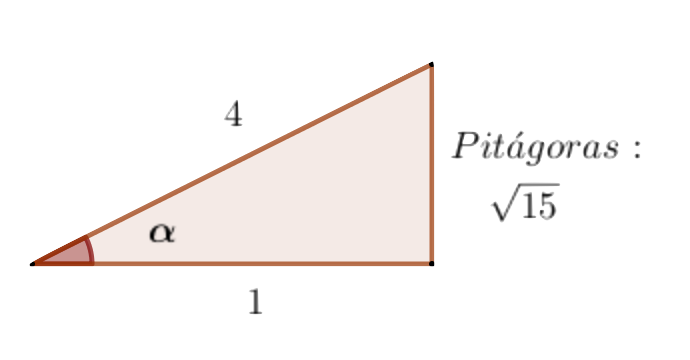
\includegraphics[width=.4\textwidth]{img-ft/ft05.png}
	\end{figure}	
\end{multicols}

Luego, $\cos \left( 2 \acos \dfrac 1 4 \right)=\cos 2\alpha=\cos^2 \alpha-\sin^2 \alpha = (1/4)^2 - (\sqrt{15}/4)^2=-7/8$
\end{miejercicio}




%*****************
\begin{miejercicio}

Calcula: $\quad \sin \left( \atan \dfrac 1 4 + \atan \dfrac 1 5 \right)$

\rule{250pt}{0.1pt}

\vspace{4mm}
Llamamos  $\ \alpha= \atan 1/4 \ \leftrightarrow \ \tan \alpha = 1/4;\quad  \beta = \atan 1/5 \ \leftrightarrow \ \tan \beta =1/5\ $ y construimos los dos triángulos de la figura, donde observamos que:

\begin{figure}[H]
	\centering
	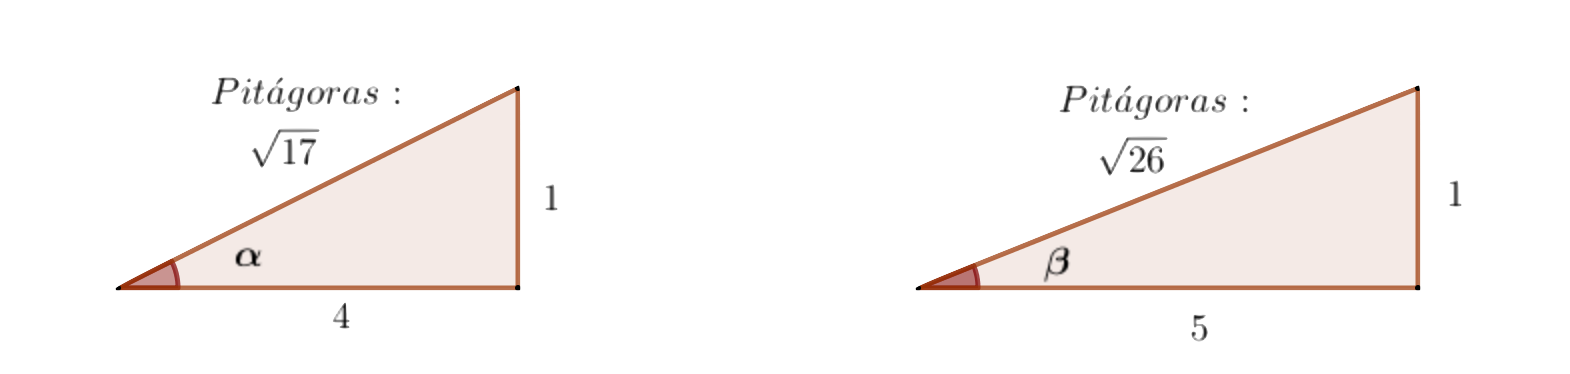
\includegraphics[width=.9\textwidth]{img-ft/ft06.png}
	\end{figure}	
$\sin \alpha= \sqrt{17}/17,\ \ \cos \alpha= 4\sqrt{17}/17;\qquad \sin \beta= \sqrt{26}/26,\ \ \cos \beta= 5\sqrt{26}/26$

\vspace{2mm} $\sin \left( \atan \dfrac 1 4 + \atan \dfrac 1 5 \right)=\sin(\alpha + \beta) = \sin \alpha \cos \beta + \cos \alpha \sin \beta =  \dfrac{\sqrt{17}}{17}\dfrac{5\sqrt{26}}{26}+\dfrac{4\sqrt{17}}{17}\dfrac{\sqrt{26}}{26}= \dfrac{9\sqrt{442}}{442}$

\end{miejercicio}


%*****************
\begin{miejercicio}

Calcula: $\quad \sin \left( 2 \acot 4 - \atan \dfrac 5{12} \right)$

\rule{250pt}{0.1pt}
\begin{figure}[H]
	\centering
	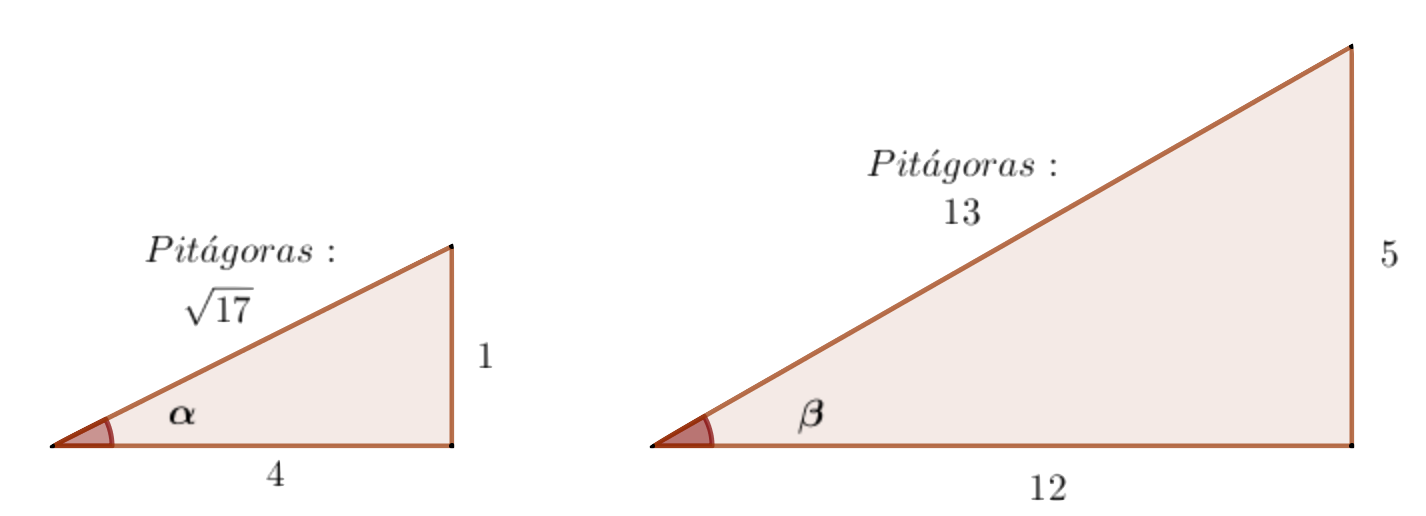
\includegraphics[width=.8\textwidth]{img-ft/ft07.png}
	\end{figure}	
Llamamos  $\ \alpha= \acot 4 \ \leftrightarrow \ \cot \alpha = 4 \ \leftrightarrow \ \tan \alpha =1/4 ;\quad  \beta = \atan 5/12 \ \leftrightarrow \ \tan \beta =5/12\ $ y construimos los dos triángulos de la figura, donde observamos que:


\vspace{2mm} $\sin \alpha= \sqrt{17}/17,\ \ \cos \alpha= 4\sqrt{17}/17;\qquad \sin \beta= 5/13,\ \ \cos \beta= 12/13$
	
\vspace{2mm} Se nos pide: $\ \sin \left( 2 \acot 4 - \atan \dfrac 5{12} \right)=\sin(2\alpha -\beta)=sin 2\alpha \cos \beta - \cos 2\alpha \sin \beta = \ \to \ (*)$

\vspace{2mm} \begin{footnotesize}
  $ \sin 2 \alpha=2\sin \alpha \cos \alpha =2  \dfrac{\sqrt{17}}{17}  \dfrac{4\sqrt{17}}{17}=\dfrac{8}{17};\quad \cos 2\alpha=\cos^2 \alpha-\sin^2 \alpha= \left(  \dfrac{\sqrt{17}}{17} \right)^2-\left(  \dfrac{4\sqrt{17}}{17} \right)^2=\dfrac{15}{17} $	
 \end{footnotesize}

\vspace{2mm}$(*)\ \to\  = \ \dfrac{8}{17}\dfrac{12}{13}-\dfrac{15}{17}\dfrac{5}{13}=\dfrac{21}{221}$ 
\end{miejercicio}




\vspace{10mm} %***********************************
%%%%%
\begin{mipropuesto}

 Comprueba: 
 
 \vspace{2mm} $a)\ \ \sin^2 \left( \dfrac{\alpha+\beta}{2} \right)-\sin^2 \left( \dfrac{\alpha-\beta}{2} \right)=\sin \alpha \, \sin \beta \, ; \quad b)\ \  \cos^2 \left( \dfrac{\alpha-\beta}{2} \right)-\cos^2 \left( \dfrac{\alpha+\beta}{2} \right)=\sin \alpha \, \sin \beta$

\end{mipropuesto}

\vspace{-8mm}
\begin{flushright}
\begin{footnotesize} \textcolor{gris}{\rotatebox{180}{ Escribe como suma por diferencia. $\quad$ a) sí; b)sí }}	\end{footnotesize}
\end{flushright}

%%%%%
\begin{mipropuesto}

 Comprueba: 
 
 \vspace{2mm}$a)\ \dfrac{\tan \alpha}{\tan 2 \alpha-\tan \alpha}=\cos 2 \alpha;\qquad b)\ \dfrac{2\sin \alpha-\sin 2 \alpha}{2\sin \alpha+\sin 2 \alpha}=\tan^2 \dfrac \alpha 2;\qquad c)\ \dfrac{\sin 2\alpha}{1+\cos 2\alpha}=\tan \alpha$ 

\end{mipropuesto}

\vspace{-8mm}
\begin{flushright}
\begin{footnotesize} \textcolor{gris}{\rotatebox{180}{ Sí, en todos los casos. }}	\end{footnotesize}
\end{flushright}


%%%%%
\begin{mipropuesto}

Simplifica: 

\vspace{2mm} $a)\ \ \dfrac{\sin 9a+\sin a}{\cos 9a-\cos a};\qquad b)\ \ \dfrac{2\cos(45+x) \cos(45-x)}{\cos 2x} ;\qquad c)\ \ \sin \theta \cos 2 \theta -\cos \theta \sin 2\theta$

\end{mipropuesto}

\vspace{-8mm}
\begin{flushright}
\begin{footnotesize} \textcolor{gris}{\rotatebox{180}{ $a) \ $ transforma en productos, $\ \cot 4a;\quad b)\ 1;\quad c)\ -\sin \theta$ }}	\end{footnotesize}
\end{flushright}


%%%%%
\begin{mipropuesto}

Resuelve: $ a)\ \ \sin 4 x -\sin 2 x =0;\qquad \qquad b)\ \cos 2x-\cos(90+x)=1$

\end{mipropuesto}

\vspace{-8mm}
\begin{flushright}
\begin{footnotesize} \textcolor{gris}{\rotatebox{180}{ $a)\ x=\{0,30,90,150,180,210,270,330\} \ (+360k) \qquad b)\ x=\{0,30,150,180\}\ (+360k)$ }}	\end{footnotesize}
\end{flushright}


%%%%%
\begin{mipropuesto}

Reseulve: $\quad a)\ \ \cos 2 x -\sin x=\sin^2 x\, ;\qquad \qquad b)\ \ 2\tan x \, \cos^2 \dfrac x 2 -\sin x=1$

\end{mipropuesto}

\vspace{-8mm}
\begin{flushright}
\begin{footnotesize} \textcolor{gris}{\rotatebox{180}{ $a)\ x=\{25.7, 154.3, 230.1, 309.9\}\ +(360k); \qquad b)\ x=\{45, 225\}\ +(360k); $ }}	\end{footnotesize}
\end{flushright}


%%%%%
\begin{mipropuesto}

Reseulve: $\quad a)\ \ \tan 2x \, \tan x=1\, ;\qquad \qquad b)\ \ \dfrac{\sin 3x+\sin x}{\cos 3x-\cos x}=\sqrt{3}$ 

\end{mipropuesto}

\vspace{-8mm}
\begin{flushright}
\begin{footnotesize} \textcolor{gris}{\rotatebox{180}{ $a)\ x=\{30,150,210,330\}\ +(360k); \quad $ Transforma en productos, $\ \ b)\ x=\{150,330\}\ +(360k)$  }}	\end{footnotesize}
\end{flushright}

%%%%%
\begin{mipropuesto}

Resuelve: $ \quad 4	\sin^2 x \cos^2 x+2\cos^2 x-2=0$

\end{mipropuesto}

\vspace{-8mm}
\begin{flushright}
\begin{footnotesize} \textcolor{gris}{\rotatebox{180}{ Bicuadrada, $\quad x=\{ \ 0,45,135,180,225,315 \ \}\ (+360k)$ }}	\end{footnotesize}
\end{flushright}

%%%%%
\begin{mipropuesto}

Reselve: $\quad a)\ \ \begin{cases} \ \sin 2 x + \cos 3 y=1 \\ \ 2\sin 2x + 4 \cos 3y=3 \end{cases}\, ; \qquad b)\ \begin{cases} \ y+\cos^2 x=1 \\ \ 2y+2\sin^2 x=0 \end{cases}$

\end{mipropuesto}

\vspace{-8mm}
\begin{flushright}
\begin{footnotesize} \textcolor{gris}{\rotatebox{180}{ $b)\ \ $ Reducción, $\ \ $ sol.: $\ y=0,\ x=\{ 0,180 \} \ (+360k)$ }}	\end{footnotesize}
\end{flushright}
\vspace{-11mm}
\begin{flushright}
\begin{footnotesize} \textcolor{gris}{\rotatebox{180}{ $\ x=\{15,75,195,255\}\ +(360k); \ \wedge \ y=\{20,100,140,220,260,340\}\ +(360k); $ independientemente. }}	\end{footnotesize}
\end{flushright}
\vspace{-11mm}
\begin{flushright}
\begin{footnotesize} \textcolor{gris}{\rotatebox{180}{ $a)\ $ Cambio variable: $\ \sin 2x=A,\ \cos 3y=B\ ; \quad $ sol.:}}	\end{footnotesize}
\end{flushright}


%%%%%
\begin{mipropuesto}

Resuelve: $\quad a)\ \ \begin{cases} \ \sin(x-y)=\sqrt{2}/2 \\ \ \sin(x+y)=\sqrt{3}/ 2 \end{cases}$ 

\end{mipropuesto}

\vspace{-8mm}
\begin{flushright}
\begin{tiny} \textcolor{gris}{\rotatebox{180}{ $(x+360k,y+360k)\ \in \
 \{ \ (52.5,7.5),\ (82.5,37.5),\ (97.5,322.5),\  (127.5,352.5),\  (232.5,187.5),\  (262.5,217.5),\  (277.5,142.5),\  (307.5,172.5) \ \}$ }}	\end{tiny}
\end{flushright}







%%%%%%%%%%%%%%%%%%%%%%%%%%%%%%%%%%%%%%%%%%%%%%%%


\newpage

%********************************************************************
\vspace{1cm}
\begin{adjustwidth}{50pt}{250pt}
\begin{cuadro-naranja}
\textbf{\huge{Problemas $\boldsymbol{+}$}}\normalsize{$\, $}
\end{cuadro-naranja}	
\end{adjustwidth}

\vspace{5mm}
\begin{enumerate}[\textbf{P$\boldsymbol +$} 1. ]

%%%%
\item	

\begin{multicols}{2}
$\quad$ 

$\quad$ Demuestra que $\ \alpha=\beta+\gamma$

$\quad$
\begin{figure}[H]
	\centering
	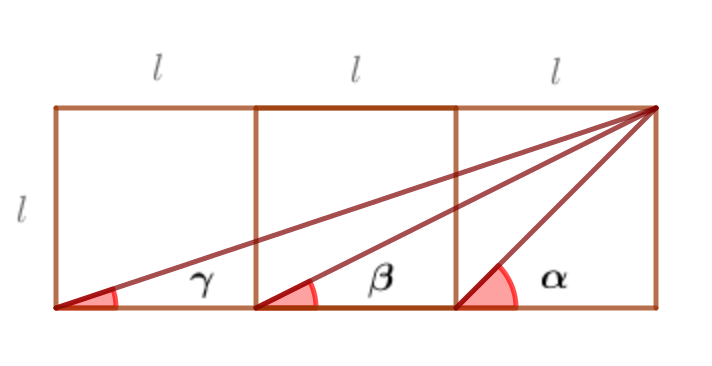
\includegraphics[width=.4\textwidth]{img-ft/ft09.png}
	\end{figure}		
\end{multicols}


\vspace{-12mm}
\begin{flushright}
\begin{footnotesize} \textcolor{gris}{\rotatebox{180}{ $\alpha,\, \beta,\, \gamma$ agudos. Basta demostrar que $\tan \alpha = \tan (\beta+\gamma)$ }}	\end{footnotesize}
\end{flushright}


%%%%
\item	Comprueba que $\quad \sin x=\dfrac {2\tan \dfrac x 2 }{1+\tan^2 \dfrac x 2}\, ; \quad \cos x =\dfrac {1-\tan^2 \dfrac x 2 }{1+\tan^2 \dfrac x 2}\, ; \quad \tan x=\dfrac {2\tan \dfrac x 2 }{1-\tan^2 \dfrac x 2}$

\vspace{-2mm}
\begin{flushright}
\begin{footnotesize} \textcolor{gris}{\rotatebox{180}{ Ysa las fórmulas del ángulo mitad. }}	\end{footnotesize}
\end{flushright}


%%%%
\item	Demuestra que existe un triángulo isósceles en el que el coseno de su ángulo desigual coincide con la suma de los cosenos de los dos ángulos iguales.

\vspace{-6mm}
\begin{flushright}
\begin{footnotesize} \textcolor{gris}{\rotatebox{180}{ $x$ ángulos iguales, $y$ ángulo desigual. $\ 2x+y=180 \ \to \ \exists x\, / \, \cos(2x-180)=2\cos x\, \ $ con $\ x<90^o$}}	\end{footnotesize}
\end{flushright}


%%%%
\item	Si $\ \alpha,\ \beta,\ \gamma $ son los ángulos de un triángulo, demuestra que 

$$ \tan \alpha + \tan \beta + \tan \gamma\ = \ \tan \alpha \cdot \tan \beta \cdot \tan \gamma  $$

\vspace{-8mm}
\begin{flushright}
\begin{footnotesize} \textcolor{gris}{\rotatebox{180}{  $\alpha+\beta+\gamma=\pi \ \to \ \gamma=\pi-(\alpha+\beta)$  }}	\end{footnotesize}
\end{flushright}




%%%%
\item	
\begin{multicols}{2}
$\quad$ 

$\quad$ ?`Qué vale $\ x+y+z\, $?

$\quad$
\begin{figure}[H]
	\centering
	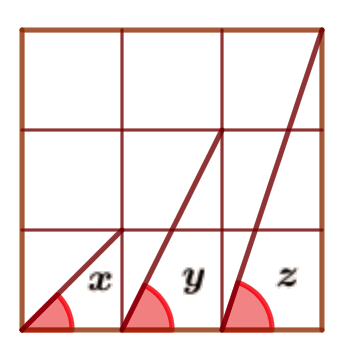
\includegraphics[width=.2\textwidth]{img-ft/ft10.png}
	\end{figure}
\end{multicols}


\vspace{-6mm}
\begin{flushright}
\begin{footnotesize} \textcolor{gris}{\rotatebox{180}{ Obviamente, $x=\pi/4$; calcula $\tan(y+z)\, , \ $ y deduce el valor de $\, y+z\, . \ $ Sol:  $\ x+y+z=\pi$ }}	\end{footnotesize}
\end{flushright}


%%%%
\item $\ \begin{cases} \ a\cos x+b\sin x &= 3 \\ \ a\sin x - b\cos x &=4 \end{cases} \quad \longrightarrow \qquad a^2\ + \ b^2 \ ?$


\vspace{-4mm}
\begin{flushright}
\begin{footnotesize} \textcolor{gris}{\rotatebox{180}{ Eleva las ecuaciones al cuadrado y súmalas. Sol.: 25. }}	\end{footnotesize}
\end{flushright}




%%%%
\item	Demuestra que $\quad \sin^2 \left( \dfrac \pi 8 - \alpha \right) - \sin^2 \left( \dfrac \pi 8 + \alpha \right) \ = \ \dfrac{\sin 2 \alpha}{\sqrt{2}}$

\vspace{-2mm}
\begin{flushright}
\begin{footnotesize} \textcolor{gris}{\rotatebox{180}{ Escribe como suma por diferencia y transforma en productos. Sol.: sí. }}	\end{footnotesize}
\end{flushright}


%%%%
\item $\ $

\begin{figure}[H]
	\centering
	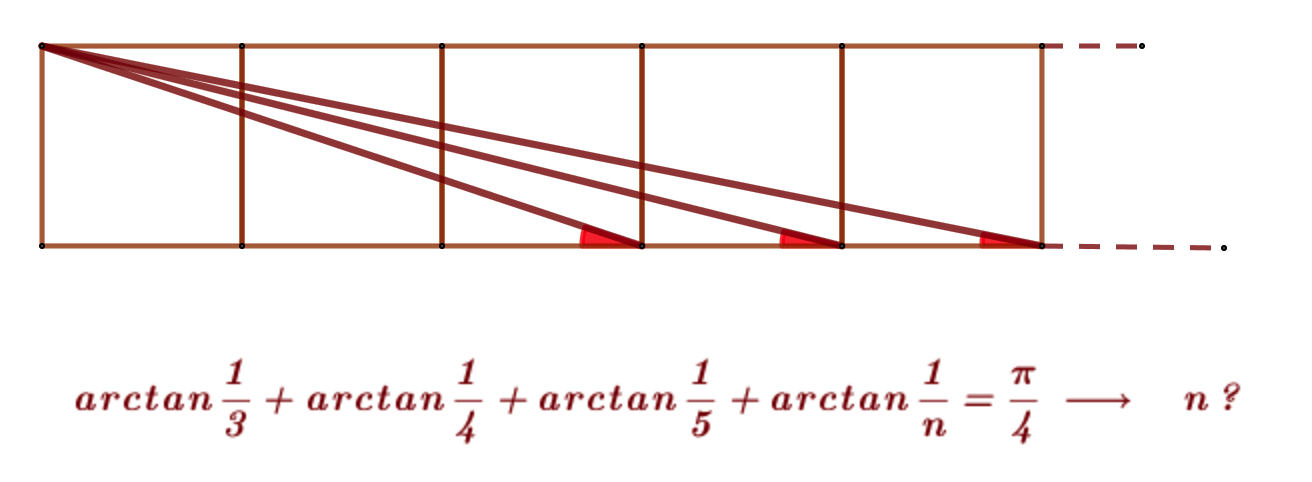
\includegraphics[width=.75\textwidth]{img-ft/ft11.png}
	\end{figure}


\vspace{-12mm}
\begin{flushright}
\begin{tiny} \textcolor{gris}{\rotatebox{180}{ $ \ \alpha+\beta+\gamma+\delta=\pi/4\  \to \ \tan(\alpha+\beta+\gamma+\delta)=\tan[\,(\alpha+\beta)\, +\, (\gamma+\delta)\, ] = \cdots $  Sol.: n=47 }}	\end{tiny}
\end{flushright}
\vspace{-11mm}
\begin{flushright}
\begin{tiny} \textcolor{gris}{\rotatebox{180}{ $\alpha=\atan 1/3,\ \beta=\atan 1/4,\ \gamma = \atan 1/5,\ \delta=\atan 1/n ,\quad $ hipótesis: }}	\end{tiny}
\end{flushright}




%%%%
\item	Resuelve: $\quad. \dfrac{\sin 3x}{\sin x}-\dfrac{\cos 3x}{\cos x}=2$

\vspace{-6mm}
\begin{flushright}
\begin{footnotesize} \textcolor{gris}{\rotatebox{180}{ Sol.:  $\forall x\in \mathbb R,\ \ $  se trata de una identidad.}}	\end{footnotesize}
\end{flushright}


%%%%
\item	Calcula: $\quad \sin(2\atan 2)-\tan \left( \dfrac \pi 4 - \atan 2 \right)$

\vspace{-6mm}
\begin{flushright}
\begin{footnotesize} \textcolor{gris}{\rotatebox{180}{ Dibuja el triángulo rectángulo adecuado y aplica fórmulas trigonométricas. Sol.: 1 }}	\end{footnotesize}
\end{flushright}


%%%%
\item	Si $\ \sin x+\cos x=1/2\, , \ $ calcula $\ \sin^3 x+\cos^3 x$

\vspace{-12mm}
\begin{flushright}
\begin{footnotesize} \textcolor{gris}{\rotatebox{180}{ Factoriza, $a^3+b^3=(a+b)(a^2-ab+b^2)$, para calcular $\sin x \cos x$ desarrollas $(\sin x+\cos x)^2$. Sol.: 11/16. }}	\end{footnotesize}
\end{flushright}



%%%%
\item	?`Cuántas soluciones tiene la ecuación $\ \sin^2 x+3\sin x \cos x+2\cos^2 x=0\, \ $ en $\ ]0,180^o[\, $?

\vspace{-6mm}
\begin{flushright}
\begin{footnotesize} \textcolor{gris}{\rotatebox{180}{ Dos, $\ 135^o\ \text{ y } \ 153.4^o$ }}	\end{footnotesize}
\end{flushright}

%%%%
\item	Simplifica: $\quad \dfrac{\sin a+ \sin 3a+ \sin 5a}{\cos a+ \cos 3a+\cos 5a}$

\vspace{-6mm}
\begin{flushright}
\begin{footnotesize} \textcolor{gris}{\rotatebox{180}{ Transforma en productos las RT de $a$ y $5a\quad $. Sol.: $\ \tan 3a$ }}	\end{footnotesize}
\end{flushright}



\end{enumerate}


\vspace{2cm}

\begin{myexampleblock}{El algoritmo de Arquímedes para el cálculo del número pi}


\small{El ingenioso método de Arquímedes para calcular el valor del número $\pi$}

\vspace{2mm}\small{El valor del número pi ($\pi$) se conoce desde la antigüedad (al menos desde el año 1800 o incluso 2000 a. C.). Por suerte también han llegado hasta nosotros los métodos que hace miles de años se emplearon para realizar los cálculos de su valor aproximado.}

\vspace{2mm}\small{Uno de los métodos más conocidos por ingenioso es el de Arquímedes de Siracusa en Los Elementos, sabía que la longitud de una circunferencia (y por tanto su relación con $\pi$) sería muy similar a la longitud de un polígono regular inscrito o cincunscrito a la misma. Cuantos más lados, más preciso sería el valor. La novedad del método de Arquímedes fue que su idea era un proceso iterativo, de modo que repitiéndolo se podían obtener valores de $\pi$ cada vez más precisos.}

\vspace{2mm}\small{Utilizó un polígono (hexágono) inscrito y otro circunscrito respecto al círculo unidad. El valor de $\pi$ quedaría por tanto entre ambos perímetros, más grande que el primero, más pequeño que el segundo. Luego repitió el proceso multiplicando por dos el número de lados: 12, 24, 48, 96, con lo que se lograba cada vez más precisión. Curiosamente al hacer esto estaba eliminando en cierto modo la geometría y convirtiéndolo todo en un procedimiento meramente aritmético.}

\vspace{2mm}\footnotesize{https://www.microsiervos.com/archivo/ciencia/ingenioso-metodo-arquimedes-calcular-numero-pi.html}


\small{La siguiente figura muestra el caso general, polígonos de $n$-lados ($n\ge 3$) y los que usó Arquímedes, partió de una hexágono y fue duplicando los lados ($6,12,24,\cdots $)}

	\begin{figure}[H]
		\centering
		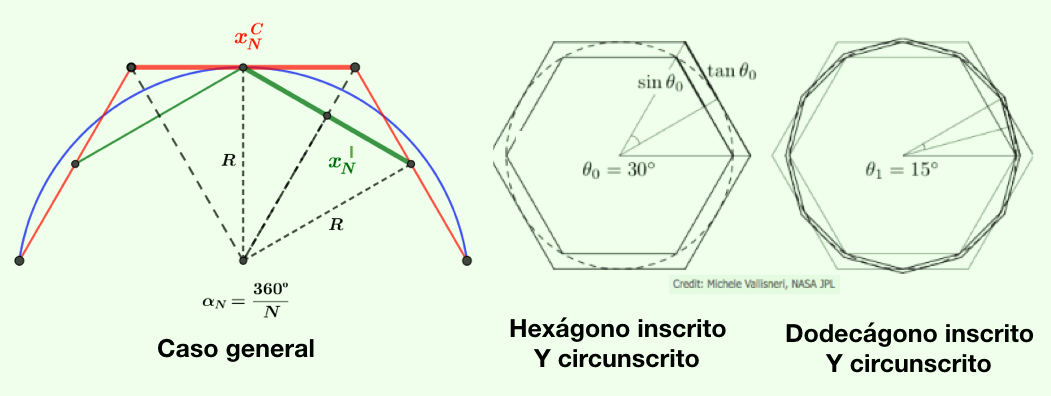
\includegraphics[width=1\textwidth]{img-ft/T01IM26.png}
	\end{figure}
	
		\noindent \small{Resolvamos el caso general y podremos particularizar para los lados que deseemos ($n \ge 3$).  Evidentemente, el ángulo central de los $n$ triángulos que aparecen tiene un valor de $\alpha_n=\dfrac {360^o}{n}$ y, según nos fijemos en el polígono circusncrito (por fuera de la circungerencia( o inscrito (por dentro), el radio de la circunferencia $R$ ($1$ si particularizamos) será o la altura del triángulo o uno de sus lados iguales, respectivamente.}
		
		\noindent \small{En la figura, hemos llamado \textcolor{verd}{$x_n^c$} y \textcolor{green}{$x_n^i$} a los lados de los polígonos circunscritos e inscritos, respectivamente. En los primeros, $R$ es la altura del triangulo y, en los inscritos, $R$ es uno de los dos lados iguales del triángulo isósceles. Haciendo uso de la trigonometría básica:}
		
	\begin{figure}[H]
		\centering
		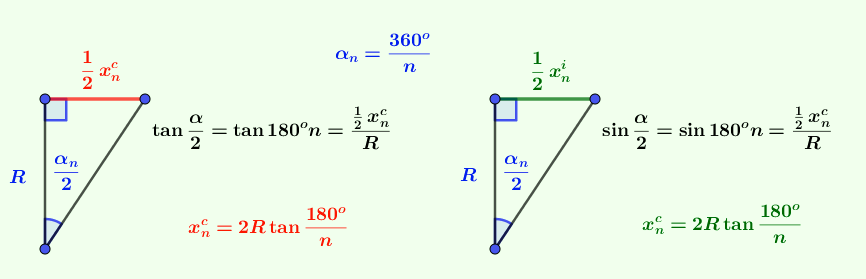
\includegraphics[width=1\textwidth]{img-ft/T01IM27.png}
	\end{figure}
	


\noindent Por lo que, el perímetro del polígono
 inscrito, $P_i$ será menor que la longitud de la circunferencia, $L$, que será  menor que	 el perímetro del polígono circunscrito, $P_c$: $\quad P_i\; <\; L \; < \; P_c\; :$
 $\; \; n \cancel{2} \bcancel{R} \sin \frac {180^o}{n} < \cancel{2} \pi \bcancel{R} < n \cancel{2} \bcancel{R} \tan \frac {180^o}{n} \longrightarrow $
 
 \noindent $\boxed{\boldsymbol{\; n\cdot \sin \frac {180^o}{n} \; <\, \pi \, < \; n\cdot \tan \frac {180^o}{n} \;}} $
 
\noindent  Relación que nos permite para cualquier polígono de $n$-lados ($n\ge 3$), obtener una aproximación por defecto y una por exeso del valor de $\pi$, que será mejor cuanto mayor sea $n$. Esto se conoce como el `método de exhaución' de Arquímedes.
 
\noindent  Con un software adecuado (p.e. una buena hoja electrónica) podemos hacer estimaciones cada vez más próximas a $\pi$ a medidsa que $n$ crece.
 
	\begin{figure}[H]
		\centering
		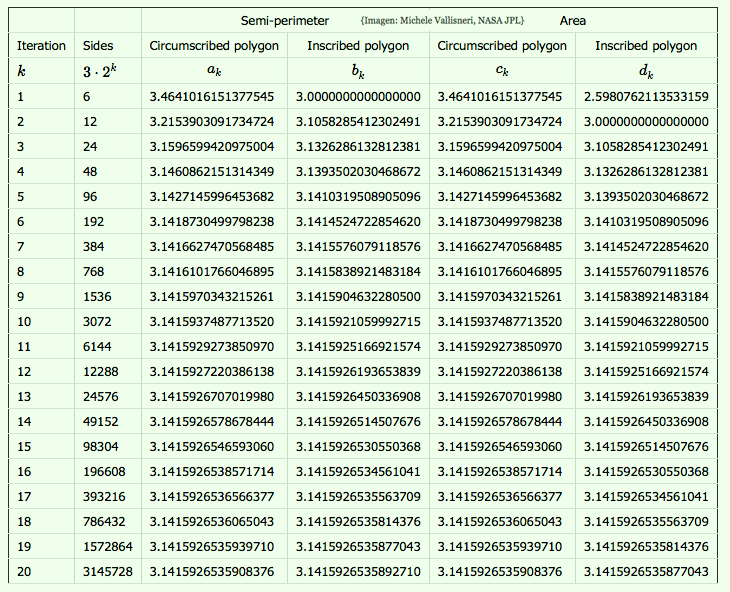
\includegraphics[width=1\textwidth]{img-ft/T01IM28.png}
	\end{figure}
	
	\noindent Podríamos haber hecho lo mismos con las áreas de los polígonos y la de la circunferencia: $A_{inscrito} < A_{círculo} < A_{circusncrito}$
	
	\noindent --- $A_{inscrito} = n \frac 1 2 x_n^i \cdot h_i = n \frac 1 2 x_n^i \sqrt{R^2-\frac 1 x (x_n^i)^2}=$
	
	\noindent  $=n \frac 1 2 2 R \sin \frac {180^o}{n}\;  \sqrt{R^2- \frac 1 4 4R^2 (\sin \frac {180^o}{n})^2}= n R^2 \sin \frac {180^o}{n}\; \sqrt{1 -(\sin \frac {180^o}{n}\;)^2}=   n R^2 \sin \frac {180^o}{n}\; \cos \frac {180^o}{n}$
	
	\noindent --- $A_{círculo}=\pi\; R^2$
	
	\noindent --- $A_{circunscrito}=n \frac 1 2 x_n^c \; R = n \frac 1 2 2 R \tan {180^o}{n}\; R = n R^2 \tan \frac {180^o}{n}$
	
 Luego: $\qquad \boxed{\;\boldsymbol{n\cdot \sin \frac {180^o}{n}\; \cos \frac {180^o}{n} \; < \; \pi \; <\; n\cdot \tan \frac {180^o}{n} } \; }$, 
	
	\noindent que es otra forma de aproximarse a $\pi$ mediante áreas en vez de perímetros.

\end{myexampleblock}
%*************************************************************

\newpage

%********************************************************************
\vspace{1cm}
\section{Resumen del tema}

\begin{tikzpicture}
	\fill [left color=red!50, right color=teal!50] (0,0) rectangle (3.5,.1);
	\fill [left color=teal!50, right color=blue!50] (3.5,0) rectangle (7.5,.1);
	\end{tikzpicture}
\vspace{0.5cm}

\begin{myblock}{Resumen \emph{``Fórmulas trigonométricas''}}

 $$\subrayado{ \ \boxed{ \  \boldsymbol{ \sin(\alpha\pm\beta)  =  \sin \alpha  \cos \beta  \pm \cos \alpha \sin \beta } } \ }  \qquad  \subrayado{ \ \boxed{ \  \boldsymbol{ \cos(\alpha \pm \beta)  =  \cos \alpha  \cos \beta   \mp  \sin \alpha  \sin \beta } } \ }$$

$$\subrayado{ \ \boxed{ \  \boldsymbol{ 
\tan (\alpha \pm \beta)  =  \dfrac {\tan \alpha \pm \tan \beta}{1 \mp \tan \alpha \, \tan \beta} } } \ }$$

\vspace{1cm}
$$\boldsymbol{
\subrayado{\boxed{ \sin 2 \alpha \ = \ 2 \, \sin \alpha \, \cos \alpha} } \qquad \qquad 
\subrayado{\boxed{ \cos 2 \alpha \ = \ \cos^2 \alpha \ - \ \sin^2 \alpha}  }}$$

\vspace{-3mm} $$\subrayado{\boldsymbol{ \boxed{ \tan 2 \alpha \ = \ \dfrac{2\, \tan \alpha}{1\, - \, \tan^2 \alpha}}}}$$


\vspace{1cm}

$$\boldsymbol{ 
\subrayado{\boxed{ \sin \dfrac \alpha 2 \ = \ \pm\sqrt{\dfrac{1-\cos \alpha}{2}} }}  \qquad 
\subrayado{\boxed{ \cos \dfrac \alpha 2 \ = \ \pm\sqrt{\dfrac{1+\cos \alpha}{2}} }}  \qquad 
\subrayado{\boxed{ \tan \dfrac \alpha 2 \ = \ \pm\sqrt{\dfrac{1-\cos \alpha}{1+\cos \alpha}} }}  
}$$

\vspace{1cm}

\begin{multicols}{2}

$\subrayado{\boxed{ \ \boldsymbol{  \sin \alpha + \sin \beta \ = \ 2 \, \sin \dfrac{\alpha + \beta}{2}\, \cos \dfrac{\alpha - \beta}{2} }  \ }}$

\vspace{3mm} $\subrayado{\boxed{ \ \boldsymbol{ \cos \alpha + \cos \beta \ = \ 2 \, \cos \dfrac{\alpha + \beta}{2}\, \cos \dfrac{\alpha - \beta}{2} }  \ }}$

$\subrayado{\boxed{ \ \boldsymbol{ \sin \alpha - \sin \beta \ = \ 2 \, \cos \dfrac{\alpha + \beta}{2}\, \sin \dfrac{\alpha - \beta}{2}  }  \ }}$

\vspace{3mm} $\subrayado{\boxed{ \ \boldsymbol{  \cos \alpha - \cos \beta \ = \ - 2 \, \sin \dfrac{\alpha + \beta}{2}\, \sin \dfrac{\alpha - \beta}{2} }  \ }}$
	
\end{multicols}
\vspace{1mm}	
\end{myblock}


\begin{comment}

%%%%%%%%%%%%%%%%%%%%%%%%%%%%%%%%%%%. SECCIONES

\begin{figure}[H]
	\centering
	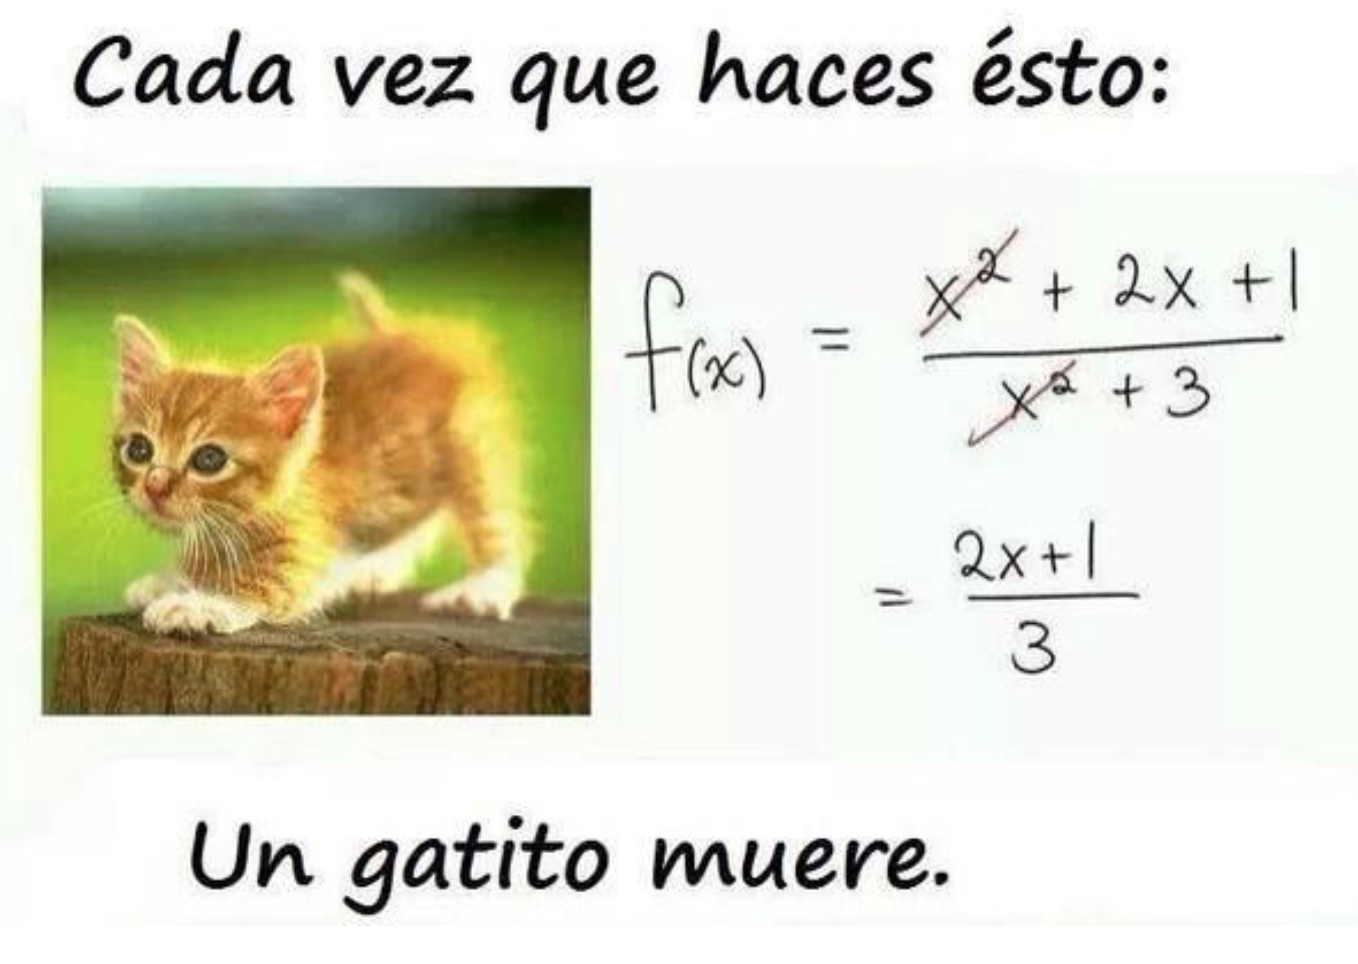
\includegraphics[width=0.35\textwidth]{img-pol/pol05.png}
\end{figure}


\chapter{texto}

\begin{tikzpicture}
	\fill [left color=red!50, right color=teal!50] (0,0) rectangle (6.5,.2);
	\fill [left color=teal!50, right color=blue!50] (6.5,0) rectangle (11.5,.2);
	\end{tikzpicture}

\vspace{1cm}
\section{texto}

\begin{tikzpicture}
	\fill [left color=red!50, right color=teal!50] (0,0) rectangle (3.5,.1);
	\fill [left color=teal!50, right color=blue!50] (3.5,0) rectangle (7.5,.1);
	\end{tikzpicture}
\vspace{0.5cm}

\subsection{texto}

\begin{tikzpicture}
	\fill [left color=red!50, right color=teal!50] (0,0) rectangle (3.5,.01);
	\fill [left color=teal!50, right color=blue!50] (3.5,0) rectangle (7.5,.01);
	\end{tikzpicture}
\vspace{0.5cm}


%%%%%%%%%%%%%%%%%%%%%%%%%%%%%%%%%%%. \begin{ ------>. 
detsacado;  cuadro-naranja;  cuadro-gris;  miejercicio (solución extensa);  mipropuesto (solución corta y fuera del cuadro)

%%%%%%%%%%%%%%%%%%%%%%%%%%%%%%%%%%%. CURIOSIDAD
\vspace{1cm}
\color{ForestGreen!80}
\rule{250pt}{0.2pt}
Texto
\vspace{-8mm}
\begin{flushright}
\rule{250pt}{0.2pt}		
\end{flushright}	
\color{black}
\end{comment}